\documentclass[12pt,fleqn,openany]{book} 

% ####
% PACOTES E DEFINIÇÕES
% ####

% ----
% Pacotes Originais do Modelo
% ----
\usepackage{comment}
\usepackage{graphicx} 
\graphicspath{{art/}} 
\usepackage{lipsum} % Inserts dummy text
\usepackage{tikz} % Required for drawing custom shapes
\usetikzlibrary{shadows}
\usetikzlibrary{fadings}
\usepackage{tcolorbox}
\tcbuselibrary{skins}
\definecolor{mygreen}{RGB}{0, 128, 0}
\usepackage{subfigure}
\usepackage{float}

\usepackage[portuguese]{babel} % English language/hyphenation
\usepackage{enumitem} % Customize lists
\setlist{nolistsep} % Reduce spacing between bullet points and numbered lists
\usepackage{booktabs} % Required for nicer horizontal rules in tables
\usepackage{xcolor} % Required for specifying colors by name
\definecolor{ocre}{RGB}{228, 104, 11} % Define the orange color used for highlighting throughout the book
\definecolor{chapterhead}{RGB}{0,156,218}
\usepackage{sectsty} %Change Color for Headings
\usepackage{indentfirst}
\usepackage{graphicx,wrapfig}
\usepackage[pt-BR]{datetime2}

% ----
% Pacotes Adicionais
% ----
\usepackage{ae}
\usepackage{lastpage}
\usepackage{mathrsfs}
\usepackage{listings}
\usepackage{multicol}
\usepackage{xspace}
\usepackage{pdflscape}
\usepackage{titlesec}
\usepackage{color, colortbl} % Para tabelas
\usepackage{epigraph} % Epígrafes e Quotes

% Configurações para tabelas
\setlength{\arrayrulewidth}{1pt}
\setlength{\tabcolsep}{18pt}
\renewcommand{\arraystretch}{1.5}

% Barras de Progresso
\usepackage[width=8cm,heightr=1,filledcolor=red,emptycolor=blue!30]{progressbar}

\usepackage{typearea} % Para anexos
\usepackage{pdfpages} % Para anexos
\usepackage{wrapfig}
\usepackage{marvosym}
\usepackage{fontawesome}
\usepackage[none]{hyphenat}

\usepackage{etoolbox} % Para Listar Ambientes
\usepackage{tabulary}
\usepackage{tabularx}
\usepackage{xcolor,soul}

\usepackage{ifthen}

\usepackage{dirtree} % Para Treeview
\usepackage{adjustbox} % Para Caixa de Cor¨

% \usepackage{draftwatermark}
% \SetWatermarkText{Rascunho} % Pacotes
% ####
% ESTRUTURA
% ####

% ----
%	MARGINS
% ----

\usepackage{geometry} % Required for adjusting page dimensions and margins

\geometry{
	paper=a4paper, % Paper size, change to letterpaper for US letter size
	top=3cm, % Top margin
	bottom=3cm, % Bottom margin
	left=3cm, % Left margin
	right=3cm, % Right margin
	headheight=14pt, % Header height
	footskip=1.4cm, % Space from the bottom margin to the baseline of the footer
	headsep=10pt, % Space from the top margin to the baseline of the header
	%showframe, % Uncomment to show how the type block is set on the page
}

% ----
%	FONTS
% ----

\usepackage{avant} % Use the Avantgarde font for headings
%\usepackage{times} % Use the Times font for headings
\usepackage{mathptmx} % Use the Adobe Times Roman as the default text font together with math symbols from the Sym­bol, Chancery and Com­puter Modern fonts

\usepackage{microtype} % Slightly tweak font spacing for aesthetics
\usepackage[utf8]{inputenc} % Required for including letters with accents
\usepackage[T1]{fontenc} % Use 8-bit encoding that has 256 glyphs
\usepackage{setspace}
\usepackage{csquotes}

% ----
%	BIBLIOGRAPHY AND INDEX
% ----

\usepackage[style=numeric,citestyle=numeric,sorting=nyt,sortcites=true,autopunct=true,babel=hyphen,hyperref=true,abbreviate=false,backref=true,backend=biber]{biblatex}
\addbibresource{refs.bib} % BibTeX bibliography file
\defbibheading{bibempty}{}

\usepackage{calc} % For simpler calculation - used for spacing the index letter headings correctly
\usepackage{makeidx} % Required to make an index
\makeindex % Tells LaTeX to create the files required for indexing

% ----
%	MAIN TABLE OF CONTENTS
% ----

\usepackage{titletoc} % Required for manipulating the table of contents

\contentsmargin{0cm} % Removes the default margin

% Part text styling (this is mostly taken care of in the PART HEADINGS section of this file)
\titlecontents{part}
	[0cm] % Left indentation
	{\addvspace{20pt}\bfseries} % Spacing and font options for parts
	{}
	{}
	{}

% Chapter text styling
\titlecontents{chapter}
	[1.25cm] % Left indentation
	{\addvspace{12pt}\large\sffamily\bfseries} % Spacing and font options for chapters
	{\color{blue!80}\contentslabel[\Large\thecontentslabel]{1.25cm}\color{blue}} % Formatting of numbered sections of this type
	{\color{blue}} % Formatting of numberless sections of this type
	{\color{blue!60}\normalsize\;\titlerule*[.5pc]{.}\;\thecontentspage} % Formatting of the filler to the right of the heading and the page number

% Section text styling
\titlecontents{section}
	[1.25cm] % Left indentation
	{\addvspace{3pt}\sffamily\bfseries} % Spacing and font options for sections
	{\contentslabel[\thecontentslabel]{1.25cm}} % Formatting of numbered sections of this type
	{} % Formatting of numberless sections of this type
	{\hfill\color{black}\thecontentspage} % Formatting of the filler to the right of the heading and the page number

% Subsection text styling
\titlecontents{subsection}
	[1.25cm] % Left indentation
	{\addvspace{1pt}\sffamily\small} % Spacing and font options for subsections
	{\contentslabel[\thecontentslabel]{1.25cm}} % Formatting of numbered sections of this type
	{} % Formatting of numberless sections of this type
	{\ \titlerule*[.5pc]{.}\;\thecontentspage} % Formatting of the filler to the right of the heading and the page number

% Subsubsection text styling
\titlecontents{subsubsection}
[1.80cm] % Left indentation
{\addvspace{1pt}\sffamily\footnotesize} % Spacing and font options for subsubsections
{\contentslabel[\thecontentslabel]{1.25cm}} % Formatting of numbered sections of this type
{} % Formatting of numberless sections of this type
{\ \titlerule*[.5pc]{.}\;\thecontentspage} % Formatting of the filler to the right of the heading and the page number

% Figure text styling
\titlecontents{figure}
	[1.25cm] % Left indentation
	{\addvspace{1pt}\sffamily\small} % Spacing and font options for figures
	{\thecontentslabel\hspace*{1em}} % Formatting of numbered sections of this type
	{} % Formatting of numberless sections of this type
	{\ \titlerule*[.5pc]{.}\;\thecontentspage} % Formatting of the filler to the right of the heading and the page number

% Table text styling
\titlecontents{table}
	[1.25cm] % Left indentation
	{\addvspace{1pt}\sffamily\small} % Spacing and font options for tables
	{\thecontentslabel\hspace*{1em}} % Formatting of numbered sections of this type
	{} % Formatting of numberless sections of this type
	{\ \titlerule*[.5pc]{.}\;\thecontentspage} % Formatting of the filler to the right of the heading and the page number

% ----
%	MINI TABLE OF CONTENTS IN PART HEADS
% ----

% Chapter text styling
\titlecontents{lchapter}
	[0em] % Left indentation
	{\addvspace{15pt}\large\sffamily\bfseries} % Spacing and font options for chapters
	{\color{blue}\contentslabel[\Large\thecontentslabel]{1.25cm}\color{blue}} % Chapter number
	{}  
	{\color{blue}\normalsize\sffamily\bfseries\;\titlerule*[.5pc]{.}\;\thecontentspage} % Page number

% Section text styling
\titlecontents{lsection}
	[0em] % Left indentation
	{\sffamily\small} % Spacing and font options for sections
	{\contentslabel[\thecontentslabel]{1.25cm}} % Section number
	{}
	{}

% Subsection text styling (note these aren't shown by default, display them by searchings this file for tocdepth and reading the commented text)
\titlecontents{lsubsection}
	[.5em] % Left indentation
	{\sffamily\footnotesize} % Spacing and font options for subsections
	{\contentslabel[\thecontentslabel]{1.25cm}}
	{}
	{}

% ----
%	HEADERS AND FOOTERS
% ----

\usepackage{fancyhdr} % Required for header and footer configuration

\pagestyle{fancy} % Enable the custom headers and footers

\renewcommand{\chaptermark}[1]{\markboth{\sffamily\normalsize\bfseries\chaptername\ \thechapter.\ #1}{}} % Styling for the current chapter in the header
\renewcommand{\sectionmark}[1]{\markright{\sffamily\normalsize\thesection\hspace{5pt}#1}{}} % Styling for the current section in the header

\newcommand{\targetR}{\hyperlink{TargetResumoAmbientes}{Resumo}}
\newcommand{\targetS}{\hyperlink{TargetTableOfContents}{Sumário}}


\fancyhf{} % Clear default headers and footers
\fancyhead[R]{\sffamily\normalsize\thepage} % Styling for the page number in the header
%\fancyhead[LO]{\rightmark} % Print the nearest section name on the left side of odd pages
%\fancyhead[RE]{\leftmark} % Print the current chapter name on the right side of even pages
%\fancyfoot[R]{\targetR} % Uncomment to include a footer
%\fancyfoot[L]{\targetS} % Uncomment to include a footer

\renewcommand{\headrulewidth}{0.5pt} % Thickness of the rule under the header

\fancypagestyle{plain}{% Style for when a plain pagestyle is specified
	\fancyhead{}\renewcommand{\headrulewidth}{0pt}%
}

% Removes the header from odd empty pages at the end of chapters
\makeatletter
\renewcommand{\cleardoublepage}{
\clearpage\ifodd\c@page\else
\hbox{}
\vspace*{\fill}
\thispagestyle{empty}
\newpage
\fi}

% ----
%	THEOREM STYLES
% ----

\usepackage{amsmath,amsfonts,amssymb,amsthm} % For math equations, theorems, symbols, etc

\newcommand{\intoo}[2]{\mathopen{]}#1\,;#2\mathclose{[}}
\newcommand{\ud}{\mathop{\mathrm{{}d}}\mathopen{}}
\newcommand{\intff}[2]{\mathopen{[}#1\,;#2\mathclose{]}}
\renewcommand{\qedsymbol}{$\blacksquare$}
\newtheorem{notation}{Notação}[chapter]

% Boxed/framed environments
\newtheoremstyle{bluenumbox}% Theorem style name
{0pt}% Space above
{0pt}% Space below
{\normalfont}% Body font
{}% Indent amount
{\small\bf\sffamily\color{blue}}% Theorem head font
{\;}% Punctuation after theorem head
{0.25em}% Space after theorem head
{\small\sffamily\color{blue}\thmname{#1}\nobreakspace\thmnumber{\@ifnotempty{#1}{}\@upn{#2}}% Theorem text (e.g. Theorem 2.1)
\thmnote{\nobreakspace\the\thm@notefont\sffamily\bfseries\color{black}---\nobreakspace#3.}} % Optional theorem note

\newtheoremstyle{blacknumex}% Theorem style name
{5pt}% Space above
{5pt}% Space below
{\normalfont}% Body font
{} % Indent amount
{\small\bf\sffamily}% Theorem head font
{\;}% Punctuation after theorem head
{0.25em}% Space after theorem head
{\small\sffamily{\tiny\ensuremath{\blacksquare}}\nobreakspace\thmname{#1}\nobreakspace\thmnumber{\@ifnotempty{#1}{}\@upn{#2}}% Theorem text (e.g. Theorem 2.1)
\thmnote{\nobreakspace\the\thm@notefont\sffamily\bfseries---\nobreakspace#3.}}% Optional theorem note

\newtheoremstyle{blacknumbox} % Theorem style name
{0pt}% Space above
{0pt}% Space below
{\normalfont}% Body font
{}% Indent amount
{\small\bf\sffamily}% Theorem head font
{\;}% Punctuation after theorem head
{0.25em}% Space after theorem head
{\small\sffamily\thmname{#1}\nobreakspace\thmnumber{\@ifnotempty{#1}{}\@upn{#2}}% Theorem text (e.g. Theorem 2.1)
\thmnote{\nobreakspace\the\thm@notefont\sffamily\bfseries---\nobreakspace#3.}}% Optional theorem note

% Non-boxed/non-framed environments
\newtheoremstyle{bluenum}% Theorem style name
{5pt}% Space above
{5pt}% Space below
{\normalfont}% Body font
{}% Indent amount
{\small\bf\sffamily\color{blue}}% Theorem head font
{\;}% Punctuation after theorem head
{0.25em}% Space after theorem head
{\small\sffamily\color{blue}\thmname{#1}\nobreakspace\thmnumber{\@ifnotempty{#1}{}\@upn{#2}}% Theorem text (e.g. Theorem 2.1)
\thmnote{\nobreakspace\the\thm@notefont\sffamily\bfseries\color{black}---\nobreakspace#3.}} % Optional theorem note
\makeatother

% Defines the theorem text style for each type of theorem to one of the three styles above
\newcounter{dummy} 
\numberwithin{dummy}{section}
\theoremstyle{bluenumbox}
\newtheorem{theoremeT}[dummy]{Teorema}
\newtheorem{problem}{Problema}[chapter]
\newtheorem{exerciseT}{Exercício}[chapter]
\theoremstyle{blacknumex}
\newtheorem{exampleT}{Exemplo}[chapter]
\theoremstyle{blacknumbox}
\newtheorem{vocabulary}{Vocabulário}[chapter]
\newtheorem{definitionT}{Definição}[section]
\newtheorem{corollaryT}[dummy]{Ação}
\theoremstyle{bluenum}
\newtheorem{proposition}[dummy]{Proposição}

% ----
%	DEFINITION OF COLORED BOXES
% ----

\RequirePackage[framemethod=default]{mdframed} % Required for creating the theorem, definition, exercise and corollary boxes

% Theorem box
\newmdenv[skipabove=7pt,
skipbelow=7pt,
backgroundcolor=black!5,
linecolor=blue,
innerleftmargin=5pt,
innerrightmargin=5pt,
innertopmargin=5pt,
leftmargin=0cm,
rightmargin=0cm,
innerbottommargin=5pt]{tBox}

% Exercise box	  
\newmdenv[skipabove=7pt,
skipbelow=7pt,
rightline=false,
leftline=true,
topline=false,
bottomline=false,
backgroundcolor=blue!10,
linecolor=blue,
innerleftmargin=5pt,
innerrightmargin=5pt,
innertopmargin=5pt,
innerbottommargin=5pt,
leftmargin=0cm,
rightmargin=0cm,
linewidth=4pt]{eBox}	

% Definition box
\newmdenv[skipabove=7pt,
skipbelow=7pt,
rightline=false,
leftline=true,
topline=false,
bottomline=false,
linecolor=blue,
innerleftmargin=5pt,
innerrightmargin=5pt,
innertopmargin=0pt,
leftmargin=0cm,
rightmargin=0cm,
linewidth=4pt,
innerbottommargin=0pt]{dBox}	

% Corollary box
\newmdenv[skipabove=7pt,
skipbelow=7pt,
rightline=false,
leftline=true,
topline=false,
bottomline=false,
linecolor=cldfC!80!black,
backgroundcolor=cldfC!40,
innerleftmargin=5pt,
innerrightmargin=5pt,
innertopmargin=5pt,
leftmargin=0cm,
rightmargin=0cm,
linewidth=4pt,
innerbottommargin=0pt,
roundcorner=10pt]{cBox}

% Creates an environment for each type of theorem and assigns it a theorem text style from the "Theorem Styles" section above and a colored box from above
\newenvironment{theorem}{\begin{tBox}\begin{theoremeT}}{\end{theoremeT}\end{tBox}}
\newenvironment{exercise}{\begin{eBox}\begin{exerciseT}}{\hfill{\color{blue}\tiny\ensuremath{\blacksquare}}\end{exerciseT}\end{eBox}}				  
\newenvironment{definition}{\begin{dBox}\begin{definitionT}}{\end{definitionT}\end{dBox}}	
\newenvironment{example}{\begin{exampleT}}{\hfill{\tiny\ensuremath{\blacksquare}}\end{exampleT}}		
\newenvironment{corollary}{\begin{cBox}\begin{corollaryT}}{\end{corollaryT}\end{cBox}}	

% ----
%	REMARK ENVIRONMENT
% ----

\newenvironment{remark}{\par\vspace{10pt}\small % Vertical white space above the remark and smaller font size
\begin{list}{}{
\leftmargin=35pt % Indentation on the left
\rightmargin=25pt}\item\ignorespaces % Indentation on the right
\makebox[-2.5pt]{\begin{tikzpicture}[overlay]
\node[draw=blue!60,line width=1pt,circle,fill=blue!25,font=\sffamily\bfseries,inner sep=2pt,outer sep=0pt] at (-15pt,0pt){\textcolor{blue}{R}};\end{tikzpicture}} % Orange R in a circle
\advance\baselineskip -1pt}{\end{list}\vskip5pt} % Tighter line spacing and white space after remark

% ----
%	SECTION NUMBERING IN THE MARGIN
% ----

\makeatletter
\renewcommand{\@seccntformat}[1]{\llap{\textcolor{blue}{\csname the#1\endcsname}\hspace{1em}}}                    
\renewcommand{\section}{\@startsection{section}{1}{\z@}
{-4ex \@plus -1ex \@minus -.4ex}
{1ex \@plus.2ex }
{\normalfont\large\sffamily\bfseries}}
\renewcommand{\subsection}{\@startsection {subsection}{2}{\z@}
{-3ex \@plus -0.1ex \@minus -.4ex}
{0.5ex \@plus.2ex }
{\normalfont\sffamily\bfseries}}
\renewcommand{\subsubsection}{\@startsection {subsubsection}{3}{\z@}
{-2ex \@plus -0.1ex \@minus -.2ex}
{.2ex \@plus.2ex }
{\normalfont\small\sffamily\bfseries}}                        
\renewcommand\paragraph{\@startsection{paragraph}{4}{\z@}
{-2ex \@plus-.2ex \@minus .2ex}
{.1ex}
{\normalfont\small\sffamily\bfseries}}

% ----
%	PART HEADINGS
% ----

% Numbered part in the table of contents
\newcommand{\@mypartnumtocformat}[2]{%
	\setlength\fboxsep{0pt}%
	\noindent\colorbox{blue!20}{\strut\parbox[c][.7cm]{\ecart}{\color{blue!70}\Large\sffamily\bfseries\centering#1}}\hskip\esp\colorbox{blue!40}{\strut\parbox[c][.7cm]{\linewidth-\ecart-\esp}{\Large\sffamily\centering#2}}%
}

% Unnumbered part in the table of contents
\newcommand{\@myparttocformat}[1]{%
	\setlength\fboxsep{0pt}%
	\noindent\colorbox{blue!40}{\strut\parbox[c][.7cm]{\linewidth}{\Large\sffamily\centering#1}}%
}

\newlength\esp
\setlength\esp{4pt}
\newlength\ecart
\setlength\ecart{1.2cm-\esp}
\newcommand{\thepartimage}{}%
\newcommand{\partimage}[1]{\renewcommand{\thepartimage}{#1}}%
\def\@part[#1]#2{%
\ifnum \c@secnumdepth >-2\relax%
\refstepcounter{part}%
\addcontentsline{toc}{part}{\texorpdfstring{\protect\@mypartnumtocformat{\thepart}{#1}}{\partname~\thepart\ ---\ #1}}
\else%
\addcontentsline{toc}{part}{\texorpdfstring{\protect\@myparttocformat{#1}}{#1}}%
\fi%
\startcontents%
\markboth{}{}%
{\thispagestyle{empty}%
\begin{tikzpicture}[remember picture,overlay]%
\node at (current page.north west){\begin{tikzpicture}[remember picture,overlay]%	
\fill[blue!20](0cm,0cm) rectangle (\paperwidth,-\paperheight);
\node[anchor=north] at (4cm,-3.25cm){\color{blue!40}\fontsize{220}{100}\sffamily\bfseries\thepart}; 
\node[anchor=south east] at (\paperwidth-1cm,-\paperheight+1cm){\parbox[t][][t]{8.5cm}{
\printcontents{l}{0}{\setcounter{tocdepth}{2}}% The depth to which the Part mini table of contents displays headings; 0 for chapters only, 1 for chapters and sections and 2 for chapters, sections and subsections
}};
\node[anchor=north east] at (\paperwidth-1.5cm,-3.25cm){\parbox[t][][t]{15cm}{\strut\raggedleft\color{white}\fontsize{30}{30}\sffamily\bfseries#2}};
\end{tikzpicture}};
\end{tikzpicture}}%
\@endpart}
\def\@spart#1{%
\startcontents%
\phantomsection
{\thispagestyle{empty}%
\begin{tikzpicture}[remember picture,overlay]%
\node at (current page.north west){\begin{tikzpicture}[remember picture,overlay]%	
\fill[blue!20](0cm,0cm) rectangle (\paperwidth,-\paperheight);
\node[anchor=north east] at (\paperwidth-1.5cm,-3.25cm){\parbox[t][][t]{15cm}{\strut\raggedleft\color{white}\fontsize{30}{30}\sffamily\bfseries#1}};
\end{tikzpicture}};
\end{tikzpicture}}
\addcontentsline{toc}{part}{\texorpdfstring{%
\setlength\fboxsep{0pt}%
\noindent\protect\colorbox{blue!40}{\strut\protect\parbox[c][.7cm]{\linewidth}{\Large\sffamily\protect\centering #1\quad\mbox{}}}}{#1}}%
\@endpart}
\def\@endpart{\vfil\newpage
\if@twoside
\if@openright
\null
\thispagestyle{empty}%
\newpage
\fi
\fi
\if@tempswa
\twocolumn
\fi}

% ----
%	CHAPTER HEADINGS
% ----

% A switch to conditionally include a picture, implemented by Christian Hupfer
\newif\ifusechapterimage
\usechapterimagetrue
\newcommand{\thechapterimage}{}%
\newcommand{\chapterimage}[1]{\ifusechapterimage\renewcommand{\thechapterimage}{#1}\fi}%
\newcommand{\autodot}{.}
\def\@makechapterhead#1{%
{\parindent \z@ \raggedright \normalfont
\ifnum \c@secnumdepth >\m@ne
\if@mainmatter
\begin{tikzpicture}[remember picture,overlay]
\node at (current page.north west)
{\begin{tikzpicture}[remember picture,overlay]
\node[anchor=north west,inner sep=0pt] at (0,0) {\ifusechapterimage\includegraphics[width=\paperwidth]{\thechapterimage}\fi};
\draw[anchor=west] (\Gm@lmargin,-9cm) node [line width=2pt,rounded corners=15pt,draw=blue,fill=white,fill opacity=0.5,inner sep=15pt]{\strut\makebox[22cm]{}};
\draw[anchor=west] (\Gm@lmargin+.3cm,-9cm) node {\huge\sffamily\bfseries\color{black}\thechapter\autodot~#1\strut};
\end{tikzpicture}};
\end{tikzpicture}
\else
\begin{tikzpicture}[remember picture,overlay]
\node at (current page.north west)
{\begin{tikzpicture}[remember picture,overlay]
\node[anchor=north west,inner sep=0pt] at (0,0) {\ifusechapterimage\includegraphics[width=\paperwidth]{\thechapterimage}\fi};
\draw[anchor=west] (\Gm@lmargin,-9cm) node [line width=2pt,rounded corners=15pt,draw=blue,fill=white,fill opacity=0.5,inner sep=15pt]{\strut\makebox[22cm]{}};
\draw[anchor=west] (\Gm@lmargin+.3cm,-9cm) node {\huge\sffamily\bfseries\color{black}#1\strut};
\end{tikzpicture}};
\end{tikzpicture}
\fi\fi\par\vspace*{270\p@}}}

%-------------------------------------------

\def\@makeschapterhead#1{%
\begin{tikzpicture}[remember picture,overlay]
\node at (current page.north west)
{\begin{tikzpicture}[remember picture,overlay]
\node[anchor=north west,inner sep=0pt] at (0,0) {\ifusechapterimage\includegraphics[width=\paperwidth]{\thechapterimage}\fi};
\draw[anchor=west] (\Gm@lmargin,-9cm) node [line width=2pt,rounded corners=15pt,draw=blue,fill=white,fill opacity=0.5,inner sep=15pt]{\strut\makebox[22cm]{}};
\draw[anchor=west] (\Gm@lmargin+.3cm,-9cm) node {\huge\sffamily\bfseries\color{black}#1\strut};
\end{tikzpicture}};
\end{tikzpicture}
\par\vspace*{270\p@}}
\makeatother

% ----
%	LINKS
% ----

\usepackage{hyperref}
\hypersetup{hidelinks,backref=true,pagebackref=true,hyperindex=true,colorlinks=false,breaklinks=true,urlcolor=blue,bookmarks=true,bookmarksopen=false}

\usepackage{bookmark}
\bookmarksetup{
open,
numbered,
addtohook={%
\ifnum\bookmarkget{level}=0 % chapter
\bookmarksetup{bold}%
\fi
\ifnum\bookmarkget{level}=-1 % part
\bookmarksetup{color=blue,bold}%
\fi
}
}

% ----
%	AMBIENTES ADICIONAIS
% ----


\newcommand{\mytitle}[1]{
    \node[left=210pt]
    at (frame.north){#1};
}

\newtcolorbox{mybox}[2][]{
    enhanced,
    overlay={\mytitle{#2}},
    borderline={2pt}{0mm}{mygreen},
    borderline={.7pt}{1mm}{mygreen},
    frame hidden,
    arc=3mm,
    sidebyside,
    lefthand width=2.5cm,
    segmentation hidden,
    top=15pt,
    left=-90pt,
    #1
}


% ATENÇÃO %

\newenvironment{aten}{\par\vspace{0pt}\small
\begin{list}{}{
\leftmargin=-15pt
\rightmargin=25pt}\item\ignorespaces 
\advance\baselineskip -1pt}{\end{list}\vskip5pt} 

\newcommand{\atencao}[1]{
\vspace{0.5cm} \begin{mybox}{\makebox[-2.5pt]{\begin{tikzpicture}[overlay]
\node at (0pt,0pt){
\includegraphics[scale=.6]{atencao}};\end{tikzpicture}}}{\begin{aten}\end{aten}}
    \tcblower
    #1
    \vspace{0.2cm}
\end{mybox}}



% SAIBA MAIS %
\newcommand{\mais}[1]{
\vspace{0.5cm} \begin{mybox}{\makebox[-2.5pt]{\begin{tikzpicture}[overlay]
\node at (0pt,0pt){
\includegraphics[scale=.6]{mais}};\end{tikzpicture}}}{\begin{aten}\end{aten}}
    \tcblower
    #1
    \vspace{0.2cm}
\end{mybox}}

% GLOSSÁRIO %
\newcommand{\glossario}[1]{
\vspace{0.5cm} \begin{mybox}{\makebox[-2.5pt]{\begin{tikzpicture}[overlay]
\node at (0pt,0pt){
\includegraphics[scale=.6]{glossario}};\end{tikzpicture}}}{\begin{aten}\end{aten}}
    \tcblower
    #1
    \vspace{0.2cm}
\end{mybox}}


% MULTIMIDIA %
\newcommand{\midia}[1]{
\vspace{0.5cm} \begin{mybox}{\makebox[-2.5pt]{\begin{tikzpicture}[overlay]
\node at (0pt,0pt){
\includegraphics[scale=.6]{midia}};\end{tikzpicture}}}{\begin{aten}\end{aten}}
    \tcblower
    #1
    \vspace{0.2cm}
\end{mybox}}

% ATIVIDADES %
\newcommand{\atividade}[1]{
\vspace{0.5cm} \begin{mybox}{\makebox[-2.5pt]{\begin{tikzpicture}[overlay]
\node at (0pt,0pt){
\includegraphics[scale=.6]{atividade}};\end{tikzpicture}}}{\begin{aten}\end{aten}}
    \tcblower
    #1
    \vspace{0.2cm}
\end{mybox}}

\setcounter{tocdepth}{3} % Profundida no Sumário

% PAGINA EM BRANCO %
\def\blankpage{%
      \clearpage%
      \thispagestyle{empty}%
      \addtocounter{page}{-1}%
      \null%
      \clearpage}
      
% NOVOS COMANDOS %
\let\parte\part
\let\capitulo\chapter
\let\secao\section
\let\subsecao\subsection
\let\subsubsecao\subsubsection

 % Estrutura
% -----------------------------------------------------------
% Comandos
% -----------------------------------------------------------
\newsavebox{\selvestebox}
\newenvironment{colbox}[1]
  {\newcommand\colboxcolor{#1}%
   \begin{lrbox}{\selvestebox}%
   \begin{minipage}{\dimexpr\columnwidth-2\fboxsep\relax}}
  {\end{minipage}\end{lrbox}%
   \begin{center}
   \colorbox[HTML]{\colboxcolor}{\usebox{\selvestebox}}
   \end{center}}

% Atentar para a ordem pois alguns comandos devem preceder outros
% -------------------------------------------------
% Cores
% -------------------------------------------------

% https://www.hexcolortool.com/F8E0E0#bded8c
\newcommand{\corTeoria}{f7b497}
\newcommand{\corExemplo}{8ce3ed}
\newcommand{\corExercicio}{e7e5e4}
\newcommand{\corNota}{ffce80}
\newcommand{\corCinza}{c5c9c6}
\newcommand{\corTodo}{9ee0ff}
\newcommand{\corCompetencia}{ADD8E6}
\newcommand{\corDefinicao}{FF7F50}

% https://www.colorhexa.com/ffb347
\newcommand{\corDestaque}{ffdca9}

% #####
% Cores do Brand book CLDF
% #####

% Cores da marca meio tom 
\definecolor{cldfA1}{RGB}{75, 87, 95} % Marrom 
\definecolor{cldfB1}{RGB}{246, 169, 36} % Laranja 
\definecolor{cldfC1}{RGB}{255, 229, 131} % Amarelo 

% Tabela Complementar
\definecolor{cldfA}{RGB}{228, 104, 11} % Laranjado
\definecolor{cldfB}{RGB}{240, 180, 80} % Amarelo
\definecolor{cldfC}{RGB}{0, 156, 218} % Azul Escuro
\definecolor{cldfD}{RGB}{89, 203, 232} % Azul Claro


\definecolor{cldfE}{RGB}{0, 144, 137} % Ciano Escuro
\definecolor{cldfF}{RGB}{110, 193, 182}  % Ciano Claro
\definecolor{cldfG}{RGB}{23, 163, 69} % Verde
\definecolor{cldfH}{RGB}{205, 205, 0} % Amarelo 

\definecolor{cldfK}{RGB}{228, 54, 137} % Rosa
\definecolor{cldfL}{RGB}{242, 168, 199} % Rosa Claro
\definecolor{cldfI}{RGB}{169, 57, 138} % Roxo
\definecolor{cldfJ}{RGB}{187, 150, 193} % Roxo Claro

% #####
% Tabelas do Texto
% #####
\definecolor{corMUST}{RGB}{228, 104, 11}
\definecolor{corSHOULD}{RGB}{240, 180, 80}
\definecolor{corCOULD}{RGB}{0, 156, 218}
\definecolor{corWOULD}{RGB}{187, 150, 193}

\definecolor{corP1}{RGB}{0, 144, 137} % Primeira Posicao
\definecolor{corP2}{RGB}{110, 193, 182} % Segunda Posicao
\definecolor{corP3}{RGB}{89, 203, 232} % Terceira Posicao
\definecolor{corPF}{RGB}{187, 150, 193} % Eliminados

\definecolor{corSIM}{RGB}{119, 221, 119} % Green
\definecolor{corNAO}{RGB}{255, 105, 97} % Red
\definecolor{corMED}{RGB}{253, 253, 150} % Amarelo


% #####
% Cores Adicionais
% #####


% https://colorhunt.co/palettes/pastel
% https://colorhunt.co/palette/ffb3b3ffdba4ffe9aec1efff
\definecolor{clPastelBlue}{HTML}{C1EFFF}
\definecolor{clPastelYellow}{HTML}{FFE9AE}
\definecolor{clPastelBrown}{HTML}{FFDBA4}
\definecolor{clPastelPink}{HTML}{FFB3B3}

% https://colorhunt.co/palettes/winter
% https://colorhunt.co/palette/002b5b2b4865256d858fe3cf
\definecolor{clWinterBlue1}{HTML}{8FE3CF}
\definecolor{clWinterBlue2}{HTML}{256D85}
\definecolor{clWinterBlue3}{HTML}{2B4865}
\definecolor{clWinterBlue4}{HTML}{002B5B}

% https://colorhunt.co/palettes/summer
% https://colorhunt.co/palette/fff5e4ffe3e1ffd1d1ff9494
\definecolor{clSummerRed1}{HTML}{FFF5E4}
\definecolor{clSummerRed2}{HTML}{FFE3E1}
\definecolor{clSummerRed3}{HTML}{FFD1D1}
\definecolor{clSummerRed4}{HTML}{FF9494}

% https://colorhunt.co/palette/eae5097dce135bb3182b7a0b
\definecolor{clNatureGreen1}{HTML}{EAE509}
\definecolor{clNatureGreen2}{HTML}{7DCE13}
\definecolor{clNatureGreen3}{HTML}{5BB318}
\definecolor{clNatureGreen4}{HTML}{2B7A0B}


% #####
% Cores Tabela Logs
% #####

\definecolor{clLogF}{HTML}{FFE9AE} % Amarelo
\definecolor{clLogA}{HTML}{7DCE13} % Verde
\definecolor{clLogB}{HTML}{FFD8A9} % Laranja
\definecolor{clLogC}{HTML}{FFB3B3} % Rosa
\definecolor{clLogD}{HTML}{FFF5E4} % Vermelho
\newcommand{\toPrev}{}
\newcommand{\toProx}{}

\newcommand{\red}[1]{\textcolor{red}{\textbf{#1}}}

\newcommand{\DV}[1]{\colorbox{orange}{\textbf{Dúvida}: #1}}

\newcommand{\WR}[1]{
	\begin{center}
		\colorbox{red}{#1}
	\end{center}
}

\newcommand{\CB}[1]{
    \begin{center}
	    \textbf{#1}
    \end{center}
}

\newcommand{\RPP}[1]{
    \begin{center}
	    \colorbox{green!10}{#1}
    \end{center}
}

\newcommand{\sigla}[1]{\textbf{\textsc{#1}}}


% ----------------------------------    
\newcounter{CounterTodo}
\setcounter{CounterTodo}{0}
\newcommand{\TODO}[2][0]
{
	\ifthenelse{#1 = 0}{\renewcommand{\auxCheck}{\msrln}}{\renewcommand{\auxCheck}{\msrls}}
	
	%\renewcommand{\toPrev}{\hyperlink{TargetTodo\arabic{CounterTodo}}{<<}}
		
	\stepcounter{CounterTodo}		
	
	\renewcommand{\auxTitulo}{\textbf{\auxCheck \xspace TODO \xspace \arabic{CounterTodo}}: \hypertarget{TargetTodo\arabic{CounterTodo}}{\nohyphens{#2}} \toPrev}
	
    \begin{center}
		\colorbox{blue!10}{\auxTitulo}
		\listcsgadd{ListaTodo}{\ifthenelse{#1 = 0}{\msrln}{\msrls} #2}	
	\end{center}
}
% -----------------------------------------------------------
\newcounter{CounterTogil}
\setcounter{CounterTogil}{0}
\newcommand{\toGil}[2][0]
{
	\ifthenelse{#1 = 0}{\renewcommand{\auxCheck}{\msrln}}{\renewcommand{\auxCheck}{\msrls}}
	
	%\renewcommand{\toPrev}{\hyperlink{TargetTogil\arabic{CounterTogil}}{<<}}
	
	\stepcounter{CounterTogil}		
	
	\renewcommand{\auxTitulo}{\textbf{\auxCheck \xspace toGil \xspace \arabic{CounterTogil}}: \hypertarget{TargetTogil\arabic{CounterTogil}}{\nohyphens{#2}} \toPrev}
	
	\begin{center}
		\colorbox{blue!10}{\auxTitulo}
		\listcsgadd{ListaTogil}{\ifthenelse{#1 = 0}{\msrln}{\msrls} #2}	
	\end{center}
}
% -----------------------------------------------------------
\newcounter{CounterTopedro}
\setcounter{CounterTopedro}{0}
\newcommand{\toPedro}[2][0]
{
	\ifthenelse{#1 = 0}{\renewcommand{\auxCheck}{\msrln}}{\renewcommand{\auxCheck}{\msrls}}
	
	%\renewcommand{\toPrev}{\hyperlink{TargetTopedro\arabic{CounterTopedro}}{<<}}
	
	\stepcounter{CounterTopedro}		
	
	\renewcommand{\auxTitulo}{\textbf{\auxCheck \xspace toPedro \xspace \arabic{CounterTopedro}}: \hypertarget{TargetTopedro\arabic{CounterTopedro}}{\nohyphens{#2}} \toPrev}
	
	\begin{center}
		\colorbox{blue!10}{\auxTitulo}
		\listcsgadd{ListaTopedro}{\ifthenelse{#1 = 0}{\msrln}{\msrls} #2}	
	\end{center}
}
% -----------------------------------------------------------

% ----------------------------------
% Comando Genérico para Imprimir Listas
% ----------------------------------

\newcommand{\printlista}[2][\\]{{
		\def\listsep{\def\listsep{#1}}
		\renewcommand{\do}[1]{\listsep ##1}
		\noindent \dolistloop#2		
}}


% -----------------------------------------------
% Colorir texto com quebra de linhas automáticas
% ------------------------------------------------

\newcommand{\ctextrgb}[3][RGB]{%
	\begingroup
	\definecolor{hlcolor}{#1}{#2}\sethlcolor{hlcolor}%
	\hl{#3}%
	\endgroup
}
%Uso: \ctextrgb[RGB]{153,221,231}{Colorido}

\newcommand{\ctextcolor}[2]{%
	\begingroup
	\colorlet{usercolor}{#1}
	\sethlcolor{usercolor}\hl{#2}%
	\endgroup
}
%Uso: \ctextcolor{orange}{Colorido}

% ----------------------------------
%           Ger Sol Unid
% ----------------------------------        

\newcommand{\GERSOLUNID}[9]{
	\def\argI{#1} 
	\def\argII{#2} 
	\def\argIII{#3} 
	\def\argIV{#4} 
	\def\argV{#5} 
	\def\argVI{#6} 
	\def\argVII{#7} 
	\def\argVIII{#8} 
	\def\argIX{#9} 
	\GERSOLUNIDCMD
}

\newcommand{\GERSOLUNIDCMD}[4]{
	% ArgI: Solicitação
	% ArgII: Unidade Solicitante
	% ArgIII: Tipo
	% ArgIV: Subtipo
	% ArgV: Prop. Numero
	% ArgVI: Prop. Ano
	% ArgVII: Comissão
	% ArgVIII: Urgente
	% ArgIX: Andamento	 
	% Arg 10 - #1: Estado
	% Arg 11 - #2: Elaborador(es) 
	% Arg 12 - #3: Revisor(es) 
	% Arg 13 - #4: Ação
\begin{center}
	\scalebox{0.8}{
	\begin{tabularx}{22cm}{|c|c|X|X|}
		\hline
		\rowcolor{yellow!70} \multicolumn{4}{|c|}{ \textbf{Gerenciar Solicitações Unidade}} \\ \hline
		
		% CABEÇALHO
		\rowcolor{yellow!20} \textbf{Solicitação} & \textbf{Estado} & \textbf{Elaborador(es)} & \textbf{Revisor(es)} \\ \hline

		% CONTEUDO
		\rowcolor{cldfG!10} \mssim \argI & #1 & #2 & #3 \\ \hline
		% -----			
	\end{tabularx}   
	} 
\end{center}
}

% ----------------------------------
%           Área de Trabalho do CL
% ----------------------------------        

\newcommand{\AREATRABCL}[9]{
	\def\argI{#1} 
	\def\argII{#2} 
	\def\argIII{#3} 
	\def\argIV{#4} 
	\def\argV{#5} 
	\def\argVI{#6} 
	\def\argVII{#7} 
	\def\argVIII{#8} 
	\def\argIX{#9} 
	\AREATRABCLCMD
}

\newcommand{\AREATRABCLCMD}[4]{
	% ArgI: Solicitação
	% ArgII: Unidade Solicitante
	% ArgIII: Tipo
	% ArgIV: Subtipo
	% ArgV: Prop. Numero
	% ArgVI: Prop. Ano
	% ArgVII: Comissão
	% ArgVIII: Urgente
	% ArgIX: Andamento	 
	% Arg 10 - #1: Estado
	% Arg 11 - #2: Elaborador(es) 
	% Arg 12 - #3: Revisor(es) 
	% Arg 13 - #4: CL
	\begin{center}
		\scalebox{0.8}{
		\begin{tabularx}{22cm}{|c|c|X|X|}
			% -----	
			\hline
			\rowcolor{orange!70} \multicolumn{4}{|c|}{\textbf{Área de Trabalho de #4}} \\ \hline
			
			% CABEÇALHO
			\rowcolor{orange!20} \textbf{Solicitação} & \textbf{Estado} & \textbf{Elaborador(es)} & \textbf{Revisor(es)} \\ \hline
			
			% CONTEUDO
			\rowcolor{cldfG!10} \mssim \argI & #1 & #2 & #3 \\ \hline
			% -----	
		\end{tabularx}
		}    
	\end{center}
}

% ----------------------------------
%           Configuração das Unidades
% ----------------------------------        

\newcommand{\CONFIGURAUNID}[5]{
	\begin{center}
	\scalebox{0.8}{
		\begin{tabularx}{\textwidth}{|c|X|}
			% -----	
			\hline
			\rowcolor{cldfA!70} \multicolumn{2}{|c|}{\textbf{Configurações da Unidade #1}} \\ \hline
			
			% CABEÇALHO
			\rowcolor{cldfA!20} & \textbf{Configuração} \\ \hline
			
			% CONTEUDO
			\rowcolor{cldfD!30} #2 & Permitir auto-atribuição de \textbf{elaboradores} \\ \hline
			\rowcolor{cldfD!30} #3 & Ao permitir auto-atribuição de \textbf{elaborador(es)}, dispensar consentimento do supervisor \\ \hline
			\rowcolor{cldfG!30} #4 & Permitir auto-atribuição de \textbf{revisor(es)} \\ \hline
			\rowcolor{cldfG!30} #5 & Ao permitir auto-atribuição de \textbf{revisor(es)}, dispensar consentimento do supervisor \\ \hline
			% -----	
		\end{tabularx}
	}    
	\end{center}
}


%% ##################################        
% ----------------------------------
%         NIVEIS EXTRAS
% ----------------------------------        
% ##################################        

% titlesec
% https://tex.stackexchange.com/questions/60209/how-to-add-an-extra-level-of-sections-with-headings-below-subsubsection


\titleclass{\subsubsubsection}{straight}[\subsection]

\newcounter{subsubsubsection}[subsubsection]
\renewcommand\thesubsubsubsection{\thesubsubsection.\arabic{subsubsubsection}}
\renewcommand\theparagraph{\thesubsubsubsection.\arabic{paragraph}} % optional; useful if paragraphs are to be numbered

\titleformat{\subsubsubsection}
  {\normalfont\normalsize\bfseries}{\thesubsubsubsection}{1em}{}
\titlespacing*{\subsubsubsection}
{0pt}{3.25ex plus 1ex minus .2ex}{1.5ex plus .2ex}

\makeatletter
\renewcommand\paragraph{\@startsection{paragraph}{5}{\z@}%
  {3.25ex \@plus1ex \@minus.2ex}%
  {-1em}%
  {\normalfont\normalsize\bfseries}}
\renewcommand\subparagraph{\@startsection{subparagraph}{6}{\parindent}%
  {3.25ex \@plus1ex \@minus .2ex}%
  {-1em}%
  {\normalfont\normalsize\bfseries}}
\def\toclevel@subsubsubsection{4}
\def\toclevel@paragraph{5}
\def\toclevel@paragraph{6}
\def\l@subsubsubsection{\@dottedtocline{4}{7em}{4em}}
\def\l@paragraph{\@dottedtocline{5}{10em}{5em}}
\def\l@subparagraph{\@dottedtocline{6}{14em}{6em}}
\makeatother

\setcounter{secnumdepth}{4}
\setcounter{tocdepth}{4} %Tem que arrumar a posição
% -----------------------------------------------------------
                % Elementos: Atores, Artefatos, Etc...
% -----------------------------------------------------------
\newcommand{\auxTitulo}{}
\newcommand{\auxCheck}{}

\newenvironment{env-definicao}
    {
        \begin{colbox}{\corDefinicao}
        \textbf{Definição:}
        \parindent12pt
        \begin{quote}
        
    }
    {   \end{quote}
        \end{colbox}
    }
% -----------------------------------------------------------
\newenvironment{env-competencia}
    {
        \begin{colbox}{\corCompetencia}
        \parindent12pt
        \begin{quote}
        
    }
    {   \end{quote}
        \end{colbox}
    }
%--------------------------------------    
\newenvironment{env-nota}
    {
        \begin{colbox}{\corNota}
        \textbf{Nota:}
        \parindent12pt
    }
    {
        \end{colbox}
    }
%--------------------------------------
\newenvironment{env-nota-i}
    {
        \begin{colbox}{\corDuvida}
        \textbf{Nota:}
        \begin{itemize}
    }
    {
        \end{itemize}
        \end{colbox}
    }
%--------------------------------------
\newenvironment{env-cinza}
    {
        \begin{colbox}{\corCinza}
        \parindent12pt
    }
    {
        \end{colbox}
    }
%--------------------------------------    
%\newcounter{envtodo}[section]
\newenvironment{envtodo}[2][]
    {
        \begin{colbox}{\corTodo}
        \refstepcounter{cmdtodo}\par\medskip
        \textbf{TODO~\thecmdtodo \xspace: ``#2''} \rmfamily
        \addcontentsline{expcmdtodo}{cmdtodo}{\protect\numberline{\thecmdtodo}#2}\par
        \parindent12pt
    }
    {
        \end{colbox}
    }    
%--------------------------------------    
\newenvironment{env-destaque}[2][]
    {
    \begin{tcolorbox}[colback=cldfA!40,colframe=cldfA!80!black,title=\textbf{\nohyphens{#2}},after skip=0.2cm,before skip=0.2cm]
    }
    {
        \end{tcolorbox}
    }
% -----------------------------------------------------------
\newenvironment{env-cor}[3][]
{
	\begin{tcolorbox}[colback=#3!40,colframe=#3!80!black,title=\textbf{\nohyphens{#2}},after skip=0.2cm,before skip=0.2cm]
	}
	{
	\end{tcolorbox}
}
% -----------------------------------------------------------
\newenvironment{env-regra}[2][]
{
	\begin{tcolorbox}[colback=cldfD!40,colframe=cldfC!80!black,title=\textbf{\nohyphens{#2}},after skip=0.2cm,before skip=0.2cm]
	\begin{center}

	}
	{
	\end{center}
	\end{tcolorbox}
}
% -----------------------------------------------------------
\newenvironment{env-aplica}[2][]
{
	\begin{tcolorbox}[colback=cldfF!40,colframe=cldfE!80!black,title=\textbf{\nohyphens{#2}},after skip=0.2cm,before skip=0.2cm]
		\begin{multicols}{2}
		\begin{itemize}
			
		}
		{
		\end{itemize}
		\end{multicols}
	\end{tcolorbox}
}
% -----------------------------------------------------------
\newenvironment{env-cenario}[2][]
    {
    \begin{tcolorbox}[colback=cldfA!40,colframe=cldfA!80!black,title=\textbf{\nohyphens{#2}},leftright skip=4cm,after skip=0.2cm,before skip=0.2cm]
    }
    {
        \end{tcolorbox}
    }
% -----------------------------------------------------------
\newenvironment{env-cenario2}[2][]
    {
    \begin{tcolorbox}[colback=cldfA!40,colframe=cldfA!80!black,title=\textbf{\nohyphens{#2}},leftright skip=2.5cm,after skip=0.2cm,before skip=0.2cm]
    }
    {
        \end{tcolorbox}
    }
% -----------------------------------------------------------
\newenvironment{env-exemplo}[2][]
    {
    \begin{tcolorbox}[colback=cldfB!40,colframe=cldfB!70!black,title=\textbf{\nohyphens{#2}},after skip=0.2cm,before skip=0.2cm]
    }
    {
        \end{tcolorbox}
    }
% -----------------------------------------------------------
\newenvironment{env-auditoria}[2][]
{
	\begin{tcolorbox}[colback=cldfA!20,colframe=cldfA!70,title=\textbf{\nohyphens{#2}},left skip=0.3cm,after skip=0.1cm,before skip=0.1cm]
	}
	{
	\end{tcolorbox}
}
% -----------------------------------------------------------
\newenvironment{env-popup}[2][]
{
	\begin{center}
		\begin{tcolorbox}[colback=cldfF!40,colframe=cldfF!70!black,title=\textbf{\nohyphens{#2}},after skip=0.2cm,before skip=0.2cm,width=10cm]
		}
		{
		\end{tcolorbox}
	\end{center}
}
% -----------------------------------------------------------
\newenvironment{env-sistemas}[2][]
    {
    \begin{tcolorbox}[colback=cldfB!40,colframe=cldfB!70!black,title=\textbf{\nohyphens{#2}},after skip=0.2cm,before skip=0.2cm]
    }
    {
        \end{tcolorbox}
    }
% -----------------------------------------------------------
\newenvironment{env-caso}[2][]
    {
    \begin{tcolorbox}[colback=cldfB!40,colframe=cldfB!70!black,title=\textbf{\nohyphens{#2}},after skip=0.2cm,before skip=0.2cm]
    }
    {
        \end{tcolorbox}
    }
% -----------------------------------------------------------
\newenvironment{env-proposta}[2][]
    {
    \begin{tcolorbox}[colback=cldfC!40,colframe=cldfC!80!black,title=\large \textbf{Ação Recomendada \xspace -- \nohyphens{#2}},after skip=0.2cm,before skip=0.2cm]
    \par\parindent12pt
    }
    {
        \end{tcolorbox}
    }
% -----------------------------------------------------------
\newcounter{CounterPergunta}
\setcounter{CounterPergunta}{0}
\newenvironment{pergunta}[2][0]
{
	\ifthenelse{#1 = 0}{\renewcommand{\auxCheck}{\msrln}}{\renewcommand{\auxCheck}{\msrls}}
	
	\stepcounter{CounterPergunta}	
	
	\renewcommand{\auxTitulo}{\hypertarget{TargetPergunta\arabic{CounterPergunta}}{\textbf{\auxCheck \xspace \nohyphens{#2}}}}
	
	\begin{tcolorbox}[colback=cldfC!40,colframe=cldfC!80!black,title=\auxTitulo,after skip=0.2cm,before skip=0.2cm]		
		
		\listcsgadd{ListaPergunta}{\ifthenelse{#1 = 0}{\msrln}{\msrls} #2}	
	}
	{
	\end{tcolorbox}
}
% -----------------------------------------------------------
\newcounter{CounterResposta}
\setcounter{CounterResposta}{0}
\newenvironment{resposta}[2][0]
{
	\ifthenelse{#1 = 0}{\renewcommand{\auxCheck}{\msrln}}{\renewcommand{\auxCheck}{\msrls}}
	
	\stepcounter{CounterResposta}	
	
	\renewcommand{\auxTitulo}{\hypertarget{TargetResposta\arabic{CounterResposta}}{\textbf{\auxCheck \xspace \nohyphens{#2}}}}
	
	\begin{tcolorbox}[colback=cldfD!40,colframe=cldfD!80!black,title=\auxTitulo,after skip=0.2cm,before skip=0.2cm]		
		
		\listcsgadd{ListaResposta}{\ifthenelse{#1 = 0}{\msrln}{\msrls} #2}	
	}
	{
	\end{tcolorbox}
}
% -----------------------------------------------------------
\newcounter{CounterRequisito}
\setcounter{CounterRequisito}{0}
\newenvironment{requisito}[2][0]
{
	\ifthenelse{#1 = 0}{\renewcommand{\auxCheck}{\msrln}}{\renewcommand{\auxCheck}{\msrls}}
	
	\stepcounter{CounterRequisito}	
	
	\renewcommand{\auxTitulo}{\hypertarget{TargetRequisito\arabic{CounterRequisito}}{\textbf{\auxCheck \xspace \nohyphens{#2}}}}
	
	\begin{tcolorbox}[colback=cldfE!40,colframe=cldfE!80!black,title=\auxTitulo,after skip=0.2cm,before skip=0.2cm]		
		
		\listcsgadd{ListaRequisito}{\ifthenelse{#1 = 0}{\msrln}{\msrls} #2}	
	}
	{
	\end{tcolorbox}
}
% -----------------------------------------------------------
\newcounter{CounterExemplo}
\setcounter{CounterExemplo}{0}
\newenvironment{exemplo}[2][0]
{
	\ifthenelse{#1 = 0}{\renewcommand{\auxCheck}{\msrln}}{\renewcommand{\auxCheck}{\msrls}}
	
	\stepcounter{CounterExemplo}	
	
	\renewcommand{\auxTitulo}{\hypertarget{TargetExemplo\arabic{CounterExemplo}}{\textbf{\auxCheck \xspace \nohyphens{#2}}}}
	
	\begin{tcolorbox}[colback=cldfD!40,colframe=cldfD!80!black,title=\auxTitulo,after skip=0.2cm,before skip=0.2cm]		
		
		\listcsgadd{ListaExemplo}{\ifthenelse{#1 = 0}{\msrln}{\msrls} #2}	
	}
	{
	\end{tcolorbox}
}
% -----------------------------------------------------------
\newcounter{CounterImportante}
\setcounter{CounterImportante}{0}
\newenvironment{importante}[2][0]
{
	\ifthenelse{#1 = 0}{\renewcommand{\auxCheck}{\msrln}}{\renewcommand{\auxCheck}{\msrls}}
	
	\stepcounter{CounterImportante}	
	
	\renewcommand{\auxTitulo}{\hypertarget{TargetImportante\arabic{CounterImportante}}{\textbf{\auxCheck \xspace \nohyphens{#2}}}}
	
	\begin{tcolorbox}[colback=cldfG!40,colframe=cldfG!80!black,title=\auxTitulo,after skip=0.2cm,before skip=0.2cm]		
	
	\listcsgadd{ListaImportante}{\ifthenelse{#1 = 0}{\msrln}{\msrls} #2}	
	}
	{
	\end{tcolorbox}
}

% -----------------------------------------------------------
\newcounter{CounterFuncionalidade}
\setcounter{CounterFuncionalidade}{0}
\newenvironment{funcionalidade}[2][0]
{
	\ifthenelse{#1 = 0}{\renewcommand{\auxCheck}{\msrln}}{\renewcommand{\auxCheck}{\msrls}}
	
	\stepcounter{CounterFuncionalidade}	
	
	\renewcommand{\auxTitulo}{\hypertarget{TargetFuncionalidade\arabic{CounterFuncionalidade}}{\textbf{\auxCheck \xspace \nohyphens{#2}}}}	
	
	
	\begin{tcolorbox}[colback=cldfJ!40,colframe=cldfJ!80!black,title=\auxTitulo,after skip=0.2cm,before skip=0.2cm]
		
	\listcsgadd{ListaFuncionalidade}{\ifthenelse{#1 = 0}{\msrln}{\msrls} #2}
	}
	{
	\end{tcolorbox}
}
% -----------------------------------------------------------
\newcounter{CounterNota}
\setcounter{CounterNota}{0}
\newenvironment{nota}[2][0]
{
	\ifthenelse{#1 = 0}{\renewcommand{\auxCheck}{\msrln}}{\renewcommand{\auxCheck}{\msrls}}
	
	\stepcounter{CounterNota}	
	
	\renewcommand{\auxTitulo}{\hypertarget{TargetNota\arabic{CounterNota}}{\textbf{\auxCheck \xspace \nohyphens{#2}}}}
	
	\begin{tcolorbox}[colback=cldfC1!40,colframe=cldfC1!50!black,title=\auxTitulo,after skip=0.2cm,before skip=0.2cm]		
		
		\listcsgadd{ListaNota}{\ifthenelse{#1 = 0}{\msrln}{\msrls} #2}	
	}
	{
	\end{tcolorbox}
}
% -----------------------------------------------------------
\newcounter{CounterFalha}
\setcounter{CounterFalha}{0}
\newenvironment{falha}[2][0]
{
	\ifthenelse{#1 = 0}{\renewcommand{\auxCheck}{\msrln \xspace Falha Pendente:   }}{\renewcommand{\auxCheck}{\msrls \xspace Falha Resolvida:}}
	
	\stepcounter{CounterFalha}	
	
	\renewcommand{\auxTitulo}{\hypertarget{TargetFalha\arabic{CounterFalha}}{\textbf{\auxCheck \nohyphens{#2}}}}
	
	\begin{tcolorbox}[colback=cldfA!20!white,colframe=cldfA!90!black,title=\auxTitulo,after skip=0.2cm,before skip=0.2cm]		
		
		\listcsgadd{ListaFalha}{\ifthenelse{#1 = 0}{\msrln}{\msrls} #2}	
	}
	{
	\end{tcolorbox}
}
% -----------------------------------------------------------
\newcounter{CounterImagine}
\setcounter{CounterImagine}{0}
\newenvironment{imagine}[2][0]
{
	\ifthenelse{#1 = 0}{\renewcommand{\auxCheck}{\msrln}}{\renewcommand{\auxCheck}{\msrls}}
	
	\stepcounter{CounterImagine}	
	
	\renewcommand{\auxTitulo}{\hypertarget{TargetImagine\arabic{CounterImagine}}{\textbf{\auxCheck \xspace \nohyphens{#2}}}}
	
	\begin{tcolorbox}[colback=cldfF!40,colframe=cldfF!80!black,title=\auxTitulo,after skip=0.2cm,before skip=0.2cm]		
		
		\listcsgadd{ListaImagine}{\ifthenelse{#1 = 0}{\msrln}{\msrls} #2}	
	}
	{
	\end{tcolorbox}
}
% -----------------------------------------------------------
\newcounter{CounterAjuste}
\setcounter{CounterAjuste}{0}
\newenvironment{ajuste}[2][0]
{
	\ifthenelse{#1 = 0}{\renewcommand{\auxCheck}{\msrln}}{\renewcommand{\auxCheck}{\msrls}}
	
	\stepcounter{CounterAjuste}	
	
	\renewcommand{\auxTitulo}{\hypertarget{TargetAjuste\arabic{CounterAjuste}}{\textbf{\auxCheck \xspace \nohyphens{#2}}}}
	
	\begin{tcolorbox}[colback=cldfF!40,colframe=cldfF!80!black,title=\auxTitulo,after skip=0.2cm,before skip=0.2cm]		
		
		\listcsgadd{ListaAjuste}{\ifthenelse{#1 = 0}{\msrln}{\msrls} #2}	
	}
	{
	\end{tcolorbox}
}
% -----------------------------------------------------------
% -----------------------------------------------------------
\newcounter{CounterEvolutivo}
\setcounter{CounterEvolutivo}{0}
\newenvironment{evolutivo}[2][0]
{
	\ifthenelse{#1 = 0}{\renewcommand{\auxCheck}{\msrln}}{\renewcommand{\auxCheck}{\msrls}}
	
	\stepcounter{CounterEvolutivo}	
	
	\renewcommand{\auxTitulo}{\hypertarget{TargetEvolutivo\arabic{CounterEvolutivo}}{\textbf{\auxCheck \xspace \nohyphens{#2}}}}
	
	\begin{tcolorbox}[colback=cldfE!40,colframe=cldfE!80!black,title=\auxTitulo,after skip=0.2cm,before skip=0.2cm]		
		
		\listcsgadd{ListaEvolutivo}{\ifthenelse{#1 = 0}{\msrln}{\msrls} #2}	
	}
	{
	\end{tcolorbox}
}
% -----------------------------------------------------------
% -----------------------------------------------------------
	% Ambientes com Contadores
% -----------------------------------------------------------
\newcounter{counterpropostanumerada}
\newenvironment{env-propostanumerada}[2][]
    {
    \refstepcounter{counterpropostanumerada}\par\medskip
    \addcontentsline{exppropostas}{counterpropostanumerada}{\protect\numberline{\thecounterpropostanumerada}#2}
    \begin{tcolorbox}[colback=cldfC!40,colframe=cldfC!80!black,title=\large \textbf{Ação Recomendada~\thecounterpropostanumerada \xspace \xspace -- \nohyphens{#2}},after skip=0.2cm,before skip=0.2cm]
    \par\parindent12pt
    }
    {
    \end{tcolorbox}
    }
% -----------------------------------------------------------




% -----------------------------------------------------------
% Comando para Enumerar Ambientes
% -----------------------------------------------------------

\newcounter{CounterCMDListarAmbiente}
\newcommand{\listarAmbiente}[2][]{
	\setcounter{CounterCMDListarAmbiente}{0}
	\begin{itemize}
		\forlistloop{\stepcounter{CounterCMDListarAmbiente} \item \hyperlink{#1\arabic{CounterCMDListarAmbiente}}}{#2}
	\end{itemize}
}






% https://tex.stackexchange.com/questions/66154/how-to-construct-a-coloured-box-with-rounded-corners

% https://www.ctan.org/pkg/tcolorbox
% -----------------------------------------------------------
                % Atalhos
% -----------------------------------------------------------

% Geral
\newcommand{\CLDF}{Câmara Legislativa do Distrito Federal \xspace}
\newcommand{\CMI}{Coordenadoria de Modernização e Informática \xspace}
\newcommand{\Gartner}{Grupo \emph{Gartner} \xspace}
\newcommand{\CDDHCEDP}{Comissão de Defesa dos Direitos Humanos, Cidadania, Ética e Decoro Parlamentar}
\newcommand{\CODEPLAN}{Companhia de Planejamento do Distrito Federal}

\newcommand{\ASSEL}{Assessoria Legislativa}
\newcommand{\CL}{consultor legislativo \xspace}
\newcommand{\CLs}{consultores legislativos \xspace}
\newcommand{\CTL}{consultor técnico-legislativo \xspace}
\newcommand{\CTLs}{consultores técnico-legislativos \xspace}

% Relatórios Nomes Simples
\newcommand{\relGMQ}{relatório ``\emph{Gartner Magic Quadrant}''} 
\newcommand{\relGCC}{relatório ``\emph{Gartner Critical Capabilities}''}  
\newcommand{\relFCM}{relatório ``\emph{The Forrester Wave Client-Managed}''} 
\newcommand{\relFVM}{relatório ``\emph{The Forrester Wave Vendor-Managed}''} 

% Relatórios Nomes Completos
\newcommand{\relatorioGMQ}{relatório ``\emph{Magic Quadrant for Analytics and Business Intelligence Platforms} 2020''} 
\newcommand{\relatorioGCC}{relatório ``\emph{Critical Capabilities for Analytics and Business Intelligence Platforms} 2020''}
\newcommand{\relatorioFVM}{relatório ``\emph{The Forrester Wave: Enterprise BI Platforms (Vendor-Managed), Q3 2019''}} 
\newcommand{\relatorioFCM}{relatório ``\emph{The Forrester Wave: Enterprise BI Platforms (Client-Managed), Q3 2019''}} 

\newcommand{\RelatorioGMQ}{Relatório ``\emph{Magic Quadrant for Analytics and Business Intelligence Platforms} 2020''} 
\newcommand{\RelatorioGCC}{Relatório ``\emph{Critical Capabilities for Analytics and Business Intelligence Platforms} 2020''}
\newcommand{\RelatorioFVM}{Relatório ``\emph{The Forrester Wave: Enterprise BI Platforms (Vendor-Managed), Q3 2019''}} 
\newcommand{\RelatorioFCM}{Relatório ``\emph{The Forrester Wave: Enterprise BI Platforms (Client-Managed), Q3 2019''}} 





% Critério MoSCoW
\newtcbox{\moscowTag}[1][red]{on line,
arc=7pt,colback=#1!80!white,colframe=#1!50!black,
before upper={\rule[-3pt]{0pt}{10pt}},boxrule=1pt,
boxsep=0pt,left=6pt,right=6pt,top=2pt,bottom=2pt}

% \colorbox{corDoFundo}{\textcolor{corDoTexto}{texto}}
\newcommand{\MUST}{\moscowTag[corMUST]{MUST}}
\newcommand{\SHOULD}{\moscowTag[corSHOULD]{SHOULD}}
\newcommand{\COULD}{\moscowTag[corCOULD]{COULD}}
\newcommand{\WOULD}{\moscowTag[corWOULD]{WOULD}}

% Botões

% Botões nos dois módulos
\newcommand{\bVisualizar}{\moscowTag[cldfG]{Visualizar}\xspace}
\newcommand{\bDetalhes}{\moscowTag[cldfG]{Detalhes}\xspace}

% Botões de Gerenciar Solicitações da Unidade
\newcommand{\bGerAtrib}{\moscowTag[cldfA]{Gerenciar Atribuições}\xspace}
\newcommand{\bGerInscricoes}{\moscowTag[cldfA]{Gerenciar Inscrições}\xspace}
\newcommand{\bInscrever}{\moscowTag[yellow]{Inscrever-se}\xspace}
\newcommand{\bEncaminhar}{\moscowTag[cldfA]{Encaminhar}\xspace}
\newcommand{\bAnalisar}{\moscowTag[cldfA]{Analisar}\xspace}

% Botões da Área de Trabalho do CL
\newcommand{\bAvaliar}{\moscowTag[cldfJ]{Avaliar}\xspace}
\newcommand{\bDesistir}{\moscowTag[cldfJ]{Desistir}\xspace}
\newcommand{\bConcluir}{\moscowTag[cldfJ]{Concluir}\xspace}

% Simulação
\newcommand{\SU}{\ctextcolor{yellow!40}{Sergio Uchoa}\xspace}
\newcommand{\SD}{\ctextcolor{yellow!50}{Samuel Duarte}\xspace}
\newcommand{\ST}{\ctextcolor{yellow!60}{Sandro Teixeira}\xspace}
\newcommand{\SQ}{\ctextcolor{yellow!70}{Sebastiao Quintana}\xspace}
\newcommand{\SC}{\ctextcolor{yellow!80}{Savio Castro}\xspace}

\newcommand{\EU}{\ctextcolor{blue!10}{Eduardo Uchoa}\xspace}
\newcommand{\ED}{\ctextcolor{blue!20}{Erick Duarte}\xspace}
\newcommand{\ET}{\ctextcolor{blue!30}{Edson Teixeira}\xspace}
\newcommand{\EQ}{\ctextcolor{blue!40}{Emerson Costa}\xspace}
\newcommand{\EC}{\ctextcolor{blue!50}{Emanuel Santos}\xspace}

\newcommand{\RU}{\ctextcolor{green!20}{Rodrigo Uchoa}\xspace}
\newcommand{\RD}{\ctextcolor{green!30}{Rafael Dias}\xspace}
\newcommand{\RT}{\ctextcolor{green!40}{Roberto Torres}\xspace}
\newcommand{\RQ}{\ctextcolor{green!50}{Renato Queiroz}\xspace}
\newcommand{\RC}{\ctextcolor{green!60}{Ricardo Castro}\xspace}

\newcommand{\SOLU}{\ctextcolor{orange!20}{CONS008-2023}\xspace}
\newcommand{\SOLD}{\ctextcolor{orange!40}{PL1700F006-2021}\xspace}
\newcommand{\SOLT}{\ctextcolor{orange!60}{DEN1994P002-2021}\xspace}




% Tabelas
\newcommand{\msnone}{\textemdash}
\newcommand{\msmark}{\checkmark}

% Cenários
\newcommand{\mssim}{\Large \Checkedbox \xspace \normalsize}
\newcommand{\msnao}{\Large  \HollowBox \xspace \normalsize}
\newcommand{\msint}{\Large  \faQuestion \xspace \normalsize}

\newtcbox{\cenarioTag}[1][red]{on line,
arc=1pt,colback=#1!80!white,colframe=#1!50!black,
before upper={\rule[-3pt]{0pt}{10pt}},boxrule=1pt,
boxsep=0pt,left=6pt,right=6pt,top=2pt,bottom=2pt}

\newcommand{\mschecksim}{\cenarioTag[corSIM]{\mssim}}
\newcommand{\mschecknao}{\cenarioTag[corNAO]{\msnao}}
\newcommand{\mscheckint}{\cenarioTag[corMED]{\msint}}


% Estados das Funcionalidades
\newcommand{\msrls}{\Large \Checkedbox \xspace \normalsize}
\newcommand{\msrln}{\Large  \HollowBox \xspace \normalsize}
\newcommand{\msrlv}{\Large  \faQuestion \xspace \normalsize}
\newcommand{\msfcs}{\cenarioTag[corSIM]{\mssim}}
\newcommand{\msfcn}{\cenarioTag[corNAO]{\msnao}}



% Metáfora do Restaurante
\newcommand{\METAFORADORESTAURANTE}{\textsc{Metáfora do Restaurante}}
\newcommand{\METAFORA}{\textsc{Metáfora}}
\newcommand{\RESTAURANTE}{\textsc{Restaurante}}
\newcommand{\CLIENTE}{\textsc{Cliente}}
\newcommand{\CLIENTES}{\textsc{Clientes}}
\newcommand{\CLIENTEDORESTAURANTE}{\textsc{Cliente do Restaurante}}
\newcommand{\PRATO}{\textsc{Prato}}
\newcommand{\PRATOS}{\textsc{Pratos}}
\newcommand{\CARDAPIO}{\textsc{Cardápio de Pratos}}
\newcommand{\LIVRODERECEITAS}{\textsc{Livro de Receitas}}
\newcommand{\RECEITA}{\textsc{Receita}}
\newcommand{\RECEITAS}{\textsc{Receitas}}
\newcommand{\INGREDIENTE}{\textsc{Ingrediente}}
\newcommand{\INGREDIENTES}{\textsc{Ingredientes}}
\newcommand{\PRODUTOR}{\textsc{Produtor de Ingrediente}}
\newcommand{\PRODUTORES}{\textsc{Produtores de Ingrediente}}
\newcommand{\DESPENSA}{\textsc{Despensa}}
\newcommand{\COZINHEIRO}{\textsc{Cozinheiro}}
\newcommand{\COZINHEIROS}{\textsc{Cozinheiros}}
\newcommand{\FOGAO}{\textsc{Fogão}}
\newcommand{\GERENTE}{\textsc{Gerente}}
\newcommand{\GERENTES}{\textsc{Gerentes}}


% Tipos de Itens para Protocolo

\newcommand{\msUnd}{\faUsers \xspace}
\newcommand{\msArt}{\faFilePictureO \xspace}
\newcommand{\msObs}{\faFileTextO \xspace}
\newcommand{\msAnd}{\faMailForward \xspace}
\newcommand{\msAct}{\faGears \xspace}


 % Comandos


\hypersetup{pdftitle={Notas Técnicas},pdfauthor={CMI}} 

%----
\begin{document}

\renewcommand{\contentsname}{Tópicos}
\renewcommand\indexname{Índice}

% Elementos Pré-Textuais

% Descomentar as 2 proximas linhas:
% ####
% CAPA
% ####

% \newcommand{\sepCapaProjeto}{Projeto Sistema ASSEL}
% \newcommand{\sepCapaTipo}{\textsc{Nota Técnica}}
% \newcommand{\sepCapaTitulo}{Especificação de formatos de arquivos suportados para upload no Sistema ASSEL}
% \newcommand{\sepCapaData}{14 de Julho de 2023}
% \newcommand{\sepCapaVersao}{V1}
% \newcommand{\sepCapaFile}{sep-capa-azul.pdf}
% \newcommand{\sepCapaCor}{blue}

% \newcommand{\sepCapaProjeto}{Projeto Sistema ASSEL}
% \newcommand{\sepCapaTipo}{\textsc{Detalhamento V4}}
% \newcommand{\sepCapaTitulo}{Gerenciar Solicitações da Unidade, 
% 	
% Área de Trabalho do CL, 
% 
% Sistema de Notificações}
% \newcommand{\sepCapaData}{27 de Setembro de 2023}
% \newcommand{\sepCapaVersao}{}
% \newcommand{\sepCapaFile}{sep-capa-amarelo.pdf}
% \newcommand{\sepCapaCor}{yellow}

% Capa: Registro de Auditoria
\newcommand{\sepCapaProjeto}{Projeto Sistema ASSEL}
\newcommand{\sepCapaTipo}{\textsc{Nota Técnica}}
\newcommand{\sepCapaTitulo}{Registro de Auditoria}
\newcommand{\sepCapaData}{07 de Novembro de 2023}
\newcommand{\sepCapaVersao}{V9}
\newcommand{\sepCapaFile}{sep-capa-vinho.pdf}
\newcommand{\sepCapaCor}{blue}

% \newcommand{\sepCapaProjeto}{Projeto Sistema ASSEL}
% \newcommand{\sepCapaTipo}{\textsc{Funcionalidades e Requisitos}}
% \newcommand{\sepCapaTitulo}{Gerenciar e Analisar Serviços
% 
% Tela da ASSEL
% }
% \newcommand{\sepCapaData}{30 de Setembro de 2022}
% \newcommand{\sepCapaVersao}{V2}
% \newcommand{\sepCapaFile}{sep-capa-verde.pdf}
% \newcommand{\sepCapaCor}{green}


% \renewcommand{\sepCapaTitulo}{Gerenciar OS ASSEL}
% \renewcommand{\sepCapaData}{18 de Julho de 2022}
% \renewcommand{\sepCapaFile}{sep-capa-verde.pdf}


% \newcommand{\sepCapaProjeto}{Projeto Sistema ASSEL}
% \newcommand{\sepCapaTipo}{\textsc{Funcionalidades e Requisitos}}
% \newcommand{\sepCapaTitulo}{Registro de Auditoria}
% \newcommand{\sepCapaData}{22 de Setembro de 2022}
% \newcommand{\sepCapaVersao}{V1}
% \newcommand{\sepCapaFile}{sep-capa-amarelo.pdf}
% \newcommand{\sepCapaCor}{yellow}


% \newcommand{\sepCapaTipo}{\textsc{Funcionalidades \& Requisitos }}
% \newcommand{\sepCapaTitulo}{Registro de Auditoria V5.1}
% \newcommand{\sepCapaData}{20 de Setembro de 2022}
% \newcommand{\sepCapaFile}{sep-capa-verde.pdf}
% \newcommand{\sepCapaCor}{green}



% \newcommand{\sepCapaTipo}{\textsc{Nota Técnica}}
% \newcommand{\sepCapaTitulo}{Mapeamento de Andamentos}
% \newcommand{\sepCapaData}{18 de Julho de 2022}
% \newcommand{\sepCapaFile}{sep-capa-azul.pdf}
% \newcommand{\sepCapaCor}{blue}


% ----
% Informações da Capa
% ----
\newcommand{\capatitulo}{
\vphantom{espaço vertical em branco}
\sepCapaProjeto

\sepCapaTipo
}

\newcommand{\capasubtitulo}{

\Huge \sepCapaTitulo \xspace \sepCapaVersao

\vphantom{\small Publicado no DCL nº 22, de 16 de março de 2021}
}

\newcommand{\capaunidade}{
%\large \red{DOCUMENTO EM ELABORAÇÃO}

\large Autor: Ronie Paulucio Porfirio

\large \sepCapaData

%\vphantom{espaço vertical em branco}
}

% ----
% Código  
% ----
\begingroup

\thispagestyle{empty} % Suppress headers and footers on the title page

\begin{tikzpicture}[remember picture,overlay]
\node[inner sep=0pt] (background) at (current page.center) 
{\includegraphics[width=\paperwidth]{\sepCapaFile}};
\draw (current page.center) node [fill=\sepCapaCor!30!white,fill opacity=0.8,text opacity=1,inner sep=1cm]{\Huge\centering\bfseries\sffamily\parbox[c][][t]
{\paperwidth}
{
\centering \capatitulo\\[15pt] % Book title
{\Large \capasubtitulo}\\[20pt] % Subtitle
{\capaunidade} % Author name
}}; 
\end{tikzpicture}

\vfill

\endgroup
 % Capa
%
\includepdf[pages=-]{cfg/creditos.pdf}

% Esses debaixo nao vai ter mesmo
% nao descomentar
%% ####
% COPYRIGHT
% ####

\newpage
~\vfill
\thispagestyle{empty}

\noindent Copyright \copyright\ 2019 John Smith\\ % Copyright notice

\noindent \textsc{Published by Publisher}\\ % Publisher

\noindent \textsc{book-website.com}\\ % URL

\noindent Licensed under the Creative Commons Attribution-NonCommercial 3.0 Unported License (the ``License''). You may not use this file except in compliance with the License. You may obtain a copy of the License at \url{http://creativecommons.org/licenses/by-nc/3.0}. Unless required by applicable law or agreed to in writing, software distributed under the License is distributed on an \textsc{``as is'' basis, without warranties or conditions of any kind}, either express or implied. See the License for the specific language governing permissions and limitations under the License.\\ % License information, replace this with your own license (if any)

\noindent \textit{First printing, March 2019} % Printing/edition date
 % Copyright
%% ####
% APRESENTAÇÃO
% ####

\newpage
~\vfill
\thispagestyle{empty}

\noindent \textsc{Curso Técnico em Eletrotécnica, Instituto Federal Fluminense - Campus Itaperuna}\\

\noindent 
Caro estudante,

Bem-vindos à disciplina de Meio Ambiente e Energias Renováveis que tratará [...] para aprofundar seus conhecimentos sobre [...] no curso Técnico em Eletrotécnica do Instituto Federal Fluminense – Campus Itaperuna.

Para que seu estudo se torne proveitoso e prazeroso, esta disciplina foi organizada em [...] capítulos, com temas e subtemas que, por sua vez, são subdivididos em seções (tópicos), atendendo aos objetivos do processo de ensino-aprendizagem.
O capítulo 1, que trata [...], procuraremos compreender [...].  No capítulo 2, descreveremos
[...]. No capítulo 3, detalharemos [...]. Finalmente, no capítulo 4 refletiremos um pouco sobre [...]. Esperamos que, até o final da disciplina vocês possam:
- Ampliar a compreensão sobre [...];
- Conhecer [...];
- Identificar os aspectos [...];
- Compreender a importância [...];
Para tanto, a metodologia das aulas [...].

Porém, antes de iniciar a leitura, gostaríamos que vocês parassem um instante para refletir sobre algumas questões [...].
Não se preocupe.  Não queremos que vocês respondam de imediato todas essas questões.  Mas esperamos que, até o final, vocês tenham respostas e também formulem outras perguntas.

Vamos, então, iniciar nossas aulas? Bons estudos!

\vspace{3cm}
\DTMlangsetup{showdayofmonth=false}
\noindent \textit{1ª Ed., \today }
\DTMlangsetup{showdayofmonth=true}
 % Apresentação

%----
%	SUMÁRIO
%----

\usechapterimagefalse % If you don't want to include a chapter image, use this to toggle images off - it can be enabled later with \usechapterimagetrue


\addtocontents{toc}{\protect\hypertarget{TargetTableOfContents}{}}
\chapterimage{capitulos.pdf}
\pagestyle{empty}
\tableofcontents
\cleardoublepage
\pagestyle{fancy}

%----
%	DESENVOLVIMENTO
%----


% \chapter{Migração de Dados}


% \newcommand{\sepCapaProjeto}{Projeto Sistema ASSEL}
% \newcommand{\sepCapaTipo}{\textsc{Funcionalidades e Requisitos}}
% \newcommand{\sepCapaTitulo}{Registro de Auditoria}
% \newcommand{\sepCapaData}{22 de Setembro de 2022}
% \newcommand{\sepCapaVersao}{V1}
% \newcommand{\sepCapaFile}{sep-capa-vinho.pdf}
% \newcommand{\sepCapaCor}{blue}

\chapter*{Alterações}

\section*{Até Julho de 2023}


\begin{itemize}
	\item \textbf{29/11/2022}: Melhor detalhamento de como o registro do evento deve ser escrito na seção ``\ref{sec-evento} \nameref{sec-evento}''/
	\item \textbf{01/12/2022}: Exemplos de cenários removidos do documento.
	Para ver exemplos consultar os BDDs desenvolvidos;
	\item \textbf{05/01/2023}: Adicionado os códigos de tela para a funcionalidade ``Administrar Configurações'';
	\item \textbf{27/05/2023}: Adicionado mais códigos de tela para a funcionalidade ``Gerenciar e Analisar Solicitações''.
	\item \textbf{10/07/2023}: Modificando os códigos de tela para as abas de análise do módulo ``Gerenciar e Analisar Solicitações''.
\end{itemize}

\section*{14/09/2023 - Versão 8}
	\begin{itemize}
		\item Resumi o histórico de alterações;
		\item Criei uma seção para conter apenas as tabelas com as siglas das telas do sistema criando subseções para cada tipo de tela.
		\item Acrescentei os códigos de tela para os módulos do Sistema de Notificações.
	\end{itemize}

\section*{24/10/2023 - Versão 9}
\begin{itemize}
	\item Acrescentei os códigos de tela para os módulo de Gerenciar Solicitações da Unidade e Área de Trabalho do CL;
	\item Acrescentei os códigos de tela para os novos modais do módulo Solicitar Ordem de Serviço;
\end{itemize}


\chapter{Registro de Auditoria}
\label{detalhes:log-auditoria}

Esse documento sugere os requisitos da funcionalidade de registro de auditoria. 

É importante ressaltar que abandonamos o termo ``log de auditoria'' de forma a não criar confusão com outros tipos de log do sistema. 

Assim, preferimos o nome ``registro de auditoria'' para estabelecer uma funcionalidade que será usada pelos administradores do sistema para rastrear as ações dos usuários de forma a facilitar a solução de problemas futuros.

\section{Modelagem do Registro de Auditoria}

De forma que a modelagem da tabela de registro de auditoria no banco de dados seja simples, o registro de auditoria deve estar em uma tabela única sem relacionamentos com nenhuma outra tabela do sistema.

Portanto, o registro de auditoria terá os seguintes atributos elencados nas próximas seções.

\subsection{timestamp}

Data e Hora completa no formato ISO8601.

\subsection{tipo}

Será um caracter que representa o tipo desse evento.

\textbf{Tipo}: 
\begin{itemize}
	\item \textbf{U}: Evento cuja origem é uma ação do usuário;
	\item \textbf{S}: Evento sem relação com usuários (gerado pelo sistema);
\end{itemize}

\subsection{ator}

Identifica o ator do evento.

\subsubsection{Tipo U}

Se o ``tipo'' for \textbf{U} então o campo ator deverá conter o nome de rede do usuário logado no sistema.

Exemplos.: ``\textbf{ronie.porfirio}'',`` \textbf{gilberto.sousa}'', ``\textbf{robson.alencar}'';

\subsubsection{Tipo S}

Se o ``tipo'' for \textbf{S} então o campo ator deverá conter o nome do módulo do sistema que gerou o evento e poderá ser:

\begin{itemize}
	\item ``\textbf{sistema.web}'': Evento tem origem no Sistema ASSEL; 
	\item ``\textbf{sistema.sei}'': Evento tem origem no módulo de integração com o SEI; 
\end{itemize}


\subsection{host}

Nome do Host ou endereço IP da máquina que o ator estava usando para acessar o sistema ou vazio caso não se aplique.

\subsection{classe}

Classe ou categoria de classificação;

É um carácter, ou seja, uma letra maiúscula, que representa a classe ou categoria desse registro e podem ser:

\textbf{Classes}:
\begin{itemize}
	\item \textbf{A - ACESSO}: Usuário obteve \sigla{a}cesso a uma tela/módulo/aba/formulário modal do sistema sem necessariamente realizar qualquer tipo de ação;
	\item \textbf{D - DADO}: Eventos no qual há alteração no banco de \textbf{d}ados;
	\item \textbf{N - NOTIFICAÇÕES}: \textbf{N}otificações emitidos pelos sistema para o usuário, que não são considerados erros;
	\item \textbf{I - INFORMAÇÃO}: Eventos \textbf{I}nformativos que não são considerados erros;
	\item \textbf{W - WARNING}: Eventos de Aviso (\textbf{w}arning) que potencialmente podem se transformar em erros;
	\item \textbf{E - ERRO}: \textbf{E}rro;
	\item \textbf{F - FATAL}: Erro \textbf{f}atal que faz o sistema parar de funcionar. Exemplo: Não conseguir acessar o SEI;
\end{itemize}

\subsection{tela}

Sigla da tela ou da funcionalidade aonde o evento ocorreu.

Serão 4 caracteres que representa a funcionalidade/tela/aba/modal/mensagem onde ocorreu o evento. 

\begin{itemize}
	\item Primeira Letra: Indica o ator que normalmente utilizaria aquela tela do sistema;
	\begin{itemize}
		\item Genérico ou \textbf{I}nício: I
		\item \textbf{S}olicitante: S
		\item \textbf{A}dministrador: A		
		\item A unidade ASS\textbf{E}L: E
		\item \textbf{M}inhas Notificações: M 
		\item \textbf{U}nidades Temáticas da ASSEL: U
		\item Área de Trabalho de Consul\textbf{t}ores Legislativos: T
		\item Migração de \textbf{D}ados: D
		\item Tela de \textbf{C}onsulta: C		
	\end{itemize}
	\item Segunda Letra: Funcionalidade
	\item Terceira Letra: Tela
	\item Quarta Letra: Aba / Modal / Mensagem
\end{itemize}

Ver seção Siglas de Telas para ver as tabelas com as siglas.

\subsection{Evento}
\label{sec-evento}

Descrição textual do evento com entidades envolvidas em chaves e objetos envolvidos em colchetes e seus IDs em parenteses quando existir. 

\begin{center}
 \Large
	Verbo de Ação + \{nome da entidade\}[texto do objeto](ID)
\end{center}

\subsubsection{Verbo de Ação}

O texto de evento deve iniciar com um verbo de ação conjugado no passado com a primeira letra em maiúscula e o restante da palavra em minúsculas. Exemplos.:  Acessou, Adicionou, Ativou, Selecionou, Vinculou, Excluiu.

\subsubsection{Nome da Entidade}
	Após o verbo de ação, deve haver um espaço e, em seguida, a entidade entre chaves em letras minúsculas. 
	
	No paradigma de orientação a objetos a entidade equivale à classe de um objeto. Em um banco de dados, a classe seria equivalente ao nome da tabela que armazena registros.      

	Alguns exemplos de entidades que deverão aparecer nos cenários de BDDs foram listados a seguir:
	
	\begin{itemize}
		\item \textbf{anexo}: Refere-se a um registro da tabela de anexos do banco de dados;

		\item \textbf{funcionalidade}: Refere-se a um registro da tabela de funcionalidades do banco de dados. \textbf{São os módulos ou telas do sistema};

		\item \textbf{minuta\_parecer}: Refere-se a um registro da tabela de minutas de pareceres do banco de dados;

		\item \textbf{ordem\_servico}: Refere-se a um registro da tabela de ordens de serviços do banco de dados;

		\item \textbf{perfil}: Refere-se a um registro da tabela de perfis do banco de dados;

		\item \textbf{solicitante}: Refere-se a um registro da tabela de solicitantes do banco de dados;

		\item \textbf{unidade}: Refere-se a um registro da tabela de unidades do banco de dados;

		\item \textbf{usuario}: Refere-se a um registro da tabela de usuários do banco de dados;

		\item \textbf{botao}: Refere-se a botões que são clicados no sistema;
		 		
		\item \textbf{modal}: Refere-se aos modais que são acessados dentro do sistema;
		
		\item \textbf{mensagem}: Refere-se às mensagens que são exibidas;
		
	\end{itemize}



\subsubsection{Texto do Objeto}
	Após o nome da entidade, em seguida sem espaços, o texto do objeto entre colchetes. 
	
	No paradigma de orientação a objetos o texto do objeto equivale ao objeto que é instanciado a partir de uma classe. Em um banco de dados, o objeto seria equivalente ao nome do registro particular de uma tabela. 
	
	O texto do objeto deve ser o mais fiel possível ao texto do registro no banco de dados ou ao do componente visual do protótipo do sistema. Ver exemplos.
	
\subsubsection{ID}
	 Finalmente, se existir e se o cenário definir, o código do registro entre parênteses. 

\subsubsection{Exemplos}

	\begin{itemize}
		\item Acessou \{funcionalidade\}[Administrar Usuários](1);	
		\item Acessou \{modal\}[Modal de Novo Usuário];	
		\item Ativou \{botao\}[Novo Usuario];	
		\item Adicionou \{unidade\}[SEASI](20);	
		\item Adicionou \{usuario\}[robson.alencar](5);	
	\end{itemize}



\section{Limpeza do Banco de Dados por período (ou número de registros)}

Sempre que o número de registros dessa tabela ultrapassar um número considerável de registros, o sistema deverá manter apenas os registros de auditoria mais recentes  (com até alguns meses de idade). Os demais dados deverão ser exportados para CSV e deletados do banco de dados.


\section{Siglas de Telas}

As tabelas abaixo apresentam as siglas possíveis até o momento.

\subsection{Telas Iniciais - I}

%\begin{table}[!h]
\begin{center}
	\begin{tabular}{|p{4cm}|p{1.3cm}|p{5cm}|p{0.8cm}|}
		\hline
		\rowcolor{corCOULD!40} \multicolumn{4}{|c|}{\Large Siglas de Telas \textbf{I}niciais do Sistema \normalsize} \\ \hline
		
		% CABEÇALHO
		\rowcolor{lightgray} Funcionalidade & Tela & Aba / Modal / Mensagem & \textbf{Sigla} \\ \hline
		% CONTEUDO
		% -----			
		\rowcolor{corSIM!30} \textbf{S}istema ASSEL & \sigla{P}rincipal & \sigla{L}ogin & \sigla{ISPL}  \\ \hline
		\rowcolor{corSIM!30} \textbf{S}istema ASSEL & \sigla{P}rincipal & \sigla{P}rincipal & \sigla{ISPP}  \\ \hline
		\rowcolor{corSIM!30} \textbf{S}istema ASSEL & Integração com o \sigla{S}EI & \sigla{P}rincipal & \sigla{ISSP}  \\ \hline
	\end{tabular}    
	%		\caption{\label{tab:auditoria:telas0} Siglas de Telas Gerais do Sistema}
\end{center}
%\end{table}

\subsection{Telas Administrativas - AX}

%\begin{table}[!h]
\begin{center}
	\begin{tabular}{|p{4cm}|p{1.3cm}|p{5cm}|p{0.8cm}|}
		\hline
		\rowcolor{corCOULD!40} \multicolumn{4}{|c|}{\Large Siglas das Telas \textbf{Administrativas} do Sistema \normalsize} \\ \hline
		
		% CABEÇALHO
		\rowcolor{lightgray} Funcionalidade & Tela & Aba / Modal / Mensagem & Sigla \\ \hline
		% CONTEUDO
		% -----			
		% Administrar Perfis
		\rowcolor{cldfB!30} \textbf{A}dministrar \sigla{P}erfis & \sigla{P}rincipal & \sigla{P}rincipal & \sigla{APPP}  \\ \hline
		\rowcolor{cldfB!30} \textbf{A}dministrar \sigla{P}erfis & \sigla{P}rincipal & Modal \sigla{N}ovo Perfil & \sigla{APPN}  \\ \hline
		\rowcolor{cldfB!30} \textbf{A}dministrar \sigla{P}erfis & \sigla{P}rincipal & Modal \sigla{V}izualizar Perfil & \sigla{APPV}  \\ \hline
		\rowcolor{cldfB!30} \textbf{A}dministrar \sigla{P}erfis & \sigla{P}rincipal & Modal Edi\sigla{t}ar Perfil & \sigla{APPT}  \\ \hline
		\rowcolor{cldfB!30} \textbf{A}dministrar \sigla{P}erfis & \sigla{P}rincipal & Mensagem Tornar Padrão \sigla{I}nterno & \sigla{APPI}  \\ \hline
		\rowcolor{cldfB!30} \textbf{A}dministrar \sigla{P}erfis & \sigla{P}rincipal & Mensagem Tornar Padrão \sigla{E}xterno & \sigla{APPE}  \\ \hline
		\rowcolor{cldfB!30} \textbf{A}dministrar \sigla{P}erfis & \sigla{P}rincipal & Mensagem E\sigla{x}cluir & \sigla{APPX}  \\ \hline
		
		
		% Administrar Usuários
		\rowcolor{cldfA!30} \textbf{A}dministrar \sigla{U}suários & \sigla{P}rincipal & \sigla{P}rincipal & \sigla{AUPP}  \\ \hline
		\rowcolor{cldfA!30} \textbf{A}dministrar \sigla{U}suários & \sigla{P}rincipal & Modal \sigla{N}ovo Usuário & \sigla{AUPN}  \\ \hline
		\rowcolor{cldfA!30} \textbf{A}dministrar \sigla{U}suários & \sigla{P}rincipal & Modal \sigla{V}isualizar Usuário & \sigla{AUPV}  \\ \hline
		\rowcolor{cldfA!30} \textbf{A}dministrar \sigla{U}suários & \sigla{P}rincipal & Modal Edi\sigla{t}ar Usuário & \sigla{AUPT}  \\ \hline
		\rowcolor{cldfA!30} \textbf{A}dministrar \sigla{U}suários & \sigla{P}rincipal & Modal Vincular Per\sigla{f}il de Usuário & \sigla{AUPF}  \\ \hline
		\rowcolor{cldfA!30} \textbf{A}dministrar \sigla{U}suários & \sigla{P}rincipal & Mensagem \sigla{A}tivar Usuário & \sigla{AUPA}  \\ \hline
		\rowcolor{cldfA!30} \textbf{A}dministrar \sigla{U}suários & \sigla{P}rincipal & Mensagem \sigla{I}nativar Usuário & \sigla{AUPI}  \\ \hline
		\rowcolor{cldfA!30} \textbf{A}dministrar \sigla{U}suários & \sigla{P}rincipal & Mensagem E\sigla{x}cluir Usuário & \sigla{AUPX}  \\ \hline
		
		% Administrar Unidades
		\rowcolor{cldfC!30} \textbf{A}dministrar U\sigla{n}idades & \sigla{P}rincipal & \sigla{P}rincipal & \sigla{ANPP}  \\ \hline
		\rowcolor{cldfC!30} \textbf{A}dministrar U\sigla{n}idades & \sigla{P}rincipal & Modal \sigla{N}ova Unidade & \sigla{ANPN}  \\ \hline
		\rowcolor{cldfC!30} \textbf{A}dministrar U\sigla{n}idades & \sigla{P}rincipal & Modal \sigla{V}isualizar Unidade & \sigla{ANPV}  \\ \hline
		\rowcolor{cldfC!30} \textbf{A}dministrar U\sigla{n}idades & \sigla{P}rincipal & Modal Edi\sigla{t}ar Unidade & \sigla{ANPT}  \\ \hline
		\rowcolor{cldfC!30} \textbf{A}dministrar U\sigla{n}idades & \sigla{P}rincipal & Mensagem E\sigla{x}cluir Unidade & \sigla{ANPX}  \\ \hline
		
		
		% Administrar Configurações
		\rowcolor{cldfK!30} \textbf{A}dministrar \sigla{C}onfigurações & \sigla{P}rincipal & \sigla{P}rincipal & \sigla{ACPP}  \\ \hline
		\rowcolor{cldfK!30} \textbf{A}dministrar \sigla{C}onfigurações & \sigla{P}rincipal & Modal Edi\sigla{t}ar Configuração & \sigla{ACPT}  \\ \hline
	\end{tabular}    
	%		\caption{\label{tab:auditoria:telas1} Siglas de Telas Administrativas}
\end{center}
%\end{table}

\subsection{Telas de Solicitantes - SO}

% \begin{table}[!h]
	\begin{center}
		\begin{tabular}{|p{4cm}|p{1.3cm}|p{5cm}|p{0.8cm}|}
			\hline
			\rowcolor{corCOULD!40} \multicolumn{4}{|c|}{\Large Siglas das Telas de \textbf{Solicitantes} do Sistema \normalsize} \\ \hline
			
			% CABEÇALHO
			\rowcolor{lightgray} Funcionalidade & Tela & Aba / Modal / Mensagem & Sigla \\ \hline
			% CONTEUDO
			% -----			
			
			% Solicitar Ordem de Serviço
			\rowcolor{cldfE!30} \textbf{S}olicitar \textbf{O}rdem de Serviço & \sigla{P}rincipal & \sigla{P}rincipal & \sigla{SOPP}  \\ \hline
			\rowcolor{cldfE!30} \textbf{S}olicitar \textbf{O}rdem de Serviço & \sigla{P}rincipal & Modal \sigla{N}ova Solicitação & \sigla{SOPN}  \\ \hline
			\rowcolor{cldfE!30} \textbf{S}olicitar \textbf{O}rdem de Serviço & \sigla{P}rincipal & Modal \sigla{V}izualizar Solicitação & \sigla{SOPV}  \\ \hline

			\rowcolor{cldfE!30} \textbf{S}olicitar \textbf{O}rdem de Serviço & \sigla{P}rincipal & Mensagem \sigla{C}ancelar Solicitação & \sigla{SOPC}  \\ \hline							

			% Novos Modais
			\rowcolor{cldfK!30} \textbf{S}olicitar \textbf{O}rdem de Serviço & \sigla{P}rincipal & Modal de \sigla{R}esolução de Pendências & \sigla{SOPR}  \\ \hline							
			
			\rowcolor{cldfK!30} \textbf{S}olicitar \textbf{O}rdem de Serviço & \sigla{P}rincipal & Modal de \sigla{D}ownload de Artefatos & \sigla{SOPD}  \\ \hline							
			
			


			
		\end{tabular}    
		% 		\caption{\label{tab:auditoria:telas2} Siglas de Telas do Solicitante}
	\end{center}
	% \end{table}

\subsection{Telas da Assessoria Legislativa (Apoio) - EO}

% \begin{table}[!h]
	\begin{center}
		\begin{tabular}{|p{4cm}|p{1.3cm}|p{5cm}|p{0.8cm}|}
			\hline
			\rowcolor{corCOULD!40} \multicolumn{4}{|c|}{\Large Siglas das Telas da \textbf{ASSEL} \normalsize} \\ \hline
			
			% CABEÇALHO
			\rowcolor{lightgray} Funcionalidade & Tela & Aba / Modal / Mensagem & Sigla \\ \hline
			% CONTEUDO
			% -----			
			
			% Gerenciar e Analisar Solicitações - Principal
			\rowcolor{cldfF!30} ASS\textbf{E}L Gerenciar e Analisar S\textbf{o}licitações  & \sigla{P}rincipal & \sigla{P}rincipal & \sigla{EOPP}  \\ \hline
			\rowcolor{cldfF!30} ASS\textbf{E}L Gerenciar e Analisar S\textbf{o}licitações  & \sigla{P}rincipal & Modal Atribuir \sigla{D}estino & \sigla{EOPD}  \\ \hline
			\rowcolor{cldfF!30} ASS\textbf{E}L Gerenciar e Analisar S\textbf{o}licitações  & \sigla{P}rincipal & Modal Atribuir \sigla{A}tribuição & \sigla{EOPA}  \\ \hline
			\rowcolor{cldfF!30} ASS\textbf{E}L Gerenciar e Analisar S\textbf{o}licitações  & \sigla{P}rincipal & Modal Atribuir A\sigla{n}álise & \sigla{EOPN}  \\ \hline
			\rowcolor{cldfF!30} ASS\textbf{E}L Gerenciar e Analisar S\textbf{o}licitações  & \sigla{P}rincipal & Modal Visualizar Andamen\sigla{t}o  & \sigla{EOPT}  \\ \hline
			
			% Gerenciar e Analisar Solicitações - Detalhes
			\rowcolor{cldfG!20} ASS\textbf{E}L Gerenciar e Analisar S\textbf{o}licitações  & \sigla{D}etalhar & \sigla{P}rincipal & \sigla{EODP}  \\ \hline
			\rowcolor{cldfH!20} ASS\textbf{E}L Gerenciar e Analisar S\textbf{o}licitações  & \sigla{A}nalisar & \sigla{P}rincipal & \sigla{EOAP}  \\ \hline
			\rowcolor{cldfH!20} ASS\textbf{E}L Gerenciar e Analisar S\textbf{o}licitações  & \sigla{A}nalisar & Aba Proprie\textbf{d}ades & \sigla{EOAD}  \\ \hline
			\rowcolor{cldfH!20} ASS\textbf{E}L Gerenciar e Analisar S\textbf{o}licitações  & \sigla{A}nalisar & Aba De\textbf{t}alhes & \sigla{EOAT}  \\ \hline
			\rowcolor{cldfH!20} ASS\textbf{E}L Gerenciar e Analisar S\textbf{o}licitações  & \sigla{A}nalisar & Aba \textbf{R}elacionamentos & \sigla{EOAR}  \\ \hline
			\rowcolor{cldfH!20} ASS\textbf{E}L Gerenciar e Analisar S\textbf{o}licitações  & \sigla{A}nalisar & Aba Adição de Arte\textbf{f}atos & \sigla{EOAF}  \\ \hline
			\rowcolor{cldfH!20} ASS\textbf{E}L Gerenciar e Analisar S\textbf{o}licitações  & \sigla{A}nalisar & Aba Enca\textbf{m}inhamento & \sigla{EOAM}  \\ \hline			
		\end{tabular}    
		% 		\caption{\label{tab:auditoria:telas3} Siglas de Telas da ASSEL}
	\end{center}
	% \end{table}


\subsection{Telas do Módulo de Minhas Notificações - MN}


%\begin{table}[!h]
\begin{center}
	\begin{tabular}{|p{4cm}|p{1.3cm}|p{5cm}|p{0.8cm}|}
		\hline
		\rowcolor{corCOULD!40} \multicolumn{4}{|c|}{\Large Siglas das Telas do Módulo de \textbf{M}inhas Notificações\normalsize} \\ \hline
		
		% CABEÇALHO
		\rowcolor{lightgray} Funcionalidade & Tela & Aba / Modal / Mensagem & Sigla \\ \hline

		% CONTEUDO
		% -----		
		
		
% Popup Filtrar
% Modal de Excluir
% Modal de Envio Manual de Notificações
% Sino de Notificações		
			
		% Módulo Minhas Notiticações
		\rowcolor{cldfH!20} Minhas \textbf{N}otificações & \sigla{P}rincipal & \sigla{P}rincipal & \sigla{MNPP}  \\ \hline


		% Visualizar
		\rowcolor{cldfA!30} Minhas \textbf{N}otificações & \sigla{P}rincipal & Modal \sigla{V}izualizar & \sigla{MNPV}  \\ \hline

		% Filtrar
		\rowcolor{cldfC!30} Minhas \textbf{N}otificações & \sigla{P}rincipal & Popup \sigla{F}iltrar & \sigla{MNPF}  \\ \hline

		% Excluir
		\rowcolor{cldfG!30} Minhas \textbf{N}otificações & \sigla{P}rincipal & Modal E\sigla{x}cluir & \sigla{MNPX}  \\ \hline

		% Envio
		\rowcolor{cldfB!30} Minhas \textbf{N}otificações & \sigla{P}rincipal & Modal de \sigla{E}nvio & \sigla{MNPE}  \\ \hline


		% Sino
		\rowcolor{cldfK!30} Minhas \textbf{N}otificações & \sigla{S}ino & \sigla{P}rincipal & \sigla{MNSP}  \\ \hline
		
	\end{tabular}    
	%		\caption{\label{tab:auditoria:telas1} Siglas de Telas Administrativas}
\end{center}
%\end{table}



\subsection{Módulos das Unidades - Gerenciar Solicitações da Unidade - UD}


%\begin{table}[!h]
\begin{center}
	\begin{tabular}{|p{4cm}|p{1.5cm}|p{4.8cm}|p{0.8cm}|}
		\hline
		\rowcolor{corCOULD!40} \multicolumn{4}{|c|}{\Large Siglas de Telas dos Módulos das \textbf{U}nidades \normalsize} \\ 
		\rowcolor{corCOULD!40} \multicolumn{4}{|c|}{\Large Gerenciar Solicitações da Uni\textbf{d}ade \normalsize} \\ \hline

		
		% CABEÇALHO
		\rowcolor{lightgray} Funcionalidade & Tela & Aba / Modal / Mensagem & Sigla \\ \hline
		
		% CONTEUDO
		% -----		
		
		% Principal
		\rowcolor{cldfF!30} Gerenciar Solicitações da \textbf{U}ni\textbf{d}ade & \sigla{P}rincipal & \sigla{P}rincipal & \sigla{UDPP}  \\ \hline
	
		% Visualizar
		\rowcolor{cldfF!30} Gerenciar Solicitações da \textbf{U}ni\textbf{d}ade & \sigla{P}rincipal & Modal \sigla{V}izualizar & \sigla{UDPV}  \\ \hline

		% Detalhes
		\rowcolor{cldfA!30} Gerenciar Solicitações da \textbf{U}ni\textbf{d}ade & \sigla{P}rincipal & Detalhes & \sigla{UDPD}  \\ \hline
				
		% Inscrever-se
		\rowcolor{cldfG!30} Gerenciar Solicitações da \textbf{U}ni\textbf{d}ade & \sigla{P}rincipal & Modal \sigla{I}nscrever-se & \sigla{UDPI}  \\ \hline

		% Classificação
		\rowcolor{cldfG!30} Gerenciar Solicitações da \textbf{U}ni\textbf{d}ade & \sigla{P}rincipal & Modal de \sigla{C}lassificação & \sigla{UDPC}  \\ \hline

		% Configurações
		\rowcolor{cldfG!30} Gerenciar Solicitações da \textbf{U}ni\textbf{d}ade & \sigla{P}rincipal & Modal de Con\sigla{f}igurações & \sigla{UDPF}  \\ \hline

		% Encaminhar
		\rowcolor{cldfG!30} Gerenciar Solicitações da \textbf{U}ni\textbf{d}ade & \sigla{P}rincipal & Modal de Enca\sigla{m}inhamento & \sigla{UDPM}  \\ \hline

		% -------------------------------------------		
		% Gerenciar Atribuições e Inscrições
		% -------------------------------------------
		\rowcolor{cldfK!30} Gerenciar Solicitações da \textbf{U}ni\textbf{d}ade & Atribuições & Aba de Gerenciamento de A\sigla{t}ribuições & \sigla{UDTT}  \\ \hline

		\rowcolor{cldfK!30} Gerenciar Solicitações da \textbf{U}ni\textbf{d}ade & Atribuições & Aba de Gerenciamento de \sigla{I}nscrições & \sigla{UDTI}  \\ \hline


		% -------------------------------------------		
		% Modal de Análise
		% -------------------------------------------

		\rowcolor{cldfH!20} Gerenciar Solicitações da \textbf{U}ni\textbf{d}ade & \sigla{A}nalisar & \textbf{P}rincipal & \sigla{UDAP}  \\ \hline

				
		\rowcolor{cldfH!20} Gerenciar Solicitações da \textbf{U}ni\textbf{d}ade & \sigla{A}nalisar & Proprie\textbf{d}ades & \sigla{UDAD}  \\ \hline
		
		\rowcolor{cldfH!20} Gerenciar Solicitações da \textbf{U}ni\textbf{d}ade & \sigla{A}nalisar & De\textbf{t}alhes & \sigla{UDAT}  \\ \hline
		
		\rowcolor{cldfH!20} Gerenciar Solicitações da \textbf{U}ni\textbf{d}ade & \sigla{A}nalisar & \textbf{R}elacionamentos & \sigla{UDAR}  \\ \hline
		
		\rowcolor{cldfH!20} Gerenciar Solicitações da \textbf{U}ni\textbf{d}ade & \sigla{A}nalisar & Anda\textbf{m}ento & \sigla{UDAM}  \\ \hline
		
		
		
	\end{tabular}    
	%		\caption{\label{tab:auditoria:telas1} Siglas de Telas Administrativas}
\end{center}
%\end{table}



\subsection{Área de Trabalho do CL - UT}

A fazer.

\subsection{Tela de Consulta - UC}

A fazer.

\subsection{Migração de Dados - MD}

A fazer.













% -------------------------------------------------------


% \part{RESUMO}

%  \chapter{Ambientes}
\newcounter{CounterAmbientes}

\TODO{Último}

\toGil{Último}

\toPedro{Último}

\begin{pergunta}{Última}
	Última
\end{pergunta}

\begin{resposta}{Última}
	Última
\end{resposta}

\begin{importante}{Última}
	Última
\end{importante}

\begin{requisito}{Última}
	Última
\end{requisito}

\begin{funcionalidade}{Última}
	Última
\end{funcionalidade}

\begin{exemplo}{Última}
	Última
\end{exemplo}

\begin{nota}{Última}
	Última
\end{nota}

\begin{imagine}{Última}
	Última
\end{imagine}

\begin{ajuste}{Último}
	Última
\end{ajuste}

\begin{falha}[1]{Último}
	Antes
	\tcblower
	Depois
\end{falha}


\begin{falha}[0]{Último}
	Antes
	\tcblower
	Depois
\end{falha}

\begin{evolutivo}[0]{Último}
	Evolutivo
\end{evolutivo}


Resumo dos principais \hypertarget{TargetResumoAmbientes}{ambientes}:

\section{Afazeres}

Afazeres é qualquer manifestação de algo que precisa ser feito em algum momento. Não sei ainda aonde se encaixa mas precisos deixar escrito para não esquecer e depois eu reavalio esse afazer.

\subsection{Gerais}

\listarAmbiente[TargetTodo]{\ListaTodo}

\subsection{Para Gilberto}

\listarAmbiente[TargetTogil]{\ListaTogil}

\subsection{Para Pedro}

\listarAmbiente[TargetTopedro]{\ListaTopedro}

\section{Perguntas}

São dúvidas e perguntas que preciso fazer para alguém me responder. Geralmente esse alguém é o Líder de Negócios ou integrantes da área de negócios.

\listarAmbiente[TargetPergunta]{\ListaPergunta}

\section{Respostas}

São respostas às perguntas. Deixo registrado.

\listarAmbiente[TargetResposta]{\ListaResposta}

\section{Importante}

Qualquer coisa que queira destacar como importante.

\listarAmbiente[TargetImportante]{\ListaImportante}

\section{Requisitos}

Nascem dentro das entrevistas.

\listarAmbiente[TargetRequisito]{\ListaRequisito}

\section{Funcionalidades}

Já são declarações mais consolidadas de coisas que precisam acontecer.

\listarAmbiente[TargetFuncionalidade]{\ListaFuncionalidade}

\section{Exemplos}

Exemplo de algo.

\listarAmbiente[TargetExemplo]{\ListaExemplo}

\section{Nota}

Notas sobre qualquer coisa.

\listarAmbiente[TargetNota]{\ListaNota}

\section{Imagine}

Descrição de uma possibilidade. Um cenário para servir de inspiração.

\listarAmbiente[TargetImagine]{\ListaImagine}


\section{Ajustes}

Preocupações relacionadas a coisas já desenvolvidas e que podem levar a erros. 

\listarAmbiente[TargetAjuste]{\ListaAjuste}


\section{Falhas}

Falhas encontradas nos testes.

\listarAmbiente[TargetFalha]{\ListaFalha}

\section{Evolutivos}

São funcionalidades evolutivas identificadas.

\listarAmbiente[TargetEvolutivo]{\ListaEvolutivo}







% \chapter{Testes}

\begin{pergunta}{Teste 1}
	Pergunta 1
\end{pergunta}

\begin{pergunta}{Teste 2}
	Pergunta 2
\end{pergunta}

\begin{pergunta}{Teste 3}
	Pergunta 3
\end{pergunta}

\begin{pergunta}{Teste 4}
	Pergunta 4
\end{pergunta}


\begin{resposta}{Teste 1}
	Resposta 5
\end{resposta}


\printlista{\perglista}

Separa

\printlista{\resplista}





% define few variables that hold some value
\def\One{this is one}
\def\Two{this is two}
\def\Three{this is three}

% add the above commands to a list named `CmdList'
\listcsgadd{CmdList}{One}
\listcsgadd{CmdList}{Two}
\listcsgadd{CmdList}{Three}

% Now loop-over them to print their values
\begin{description}
	\renewcommand*{\do}[1]{\item[#1:] \csuse{#1}}
	\dolistcsloop{CmdList}
\end{description}    

% creating a table needs little bit more trickery; You cannot insert table entries directly.
% You first have to accumulate all table data into some temporary variable and then use that.
\begingroup
\newcommand\tablecontent{}
\def\do#1{\appto\tablecontent{\hline \textbf{#1} & \csuse{#1}\\}}%
\dolistcsloop{CmdList} % collect the data in a table format
\begin{tabulary}{\textwidth}{|L|L|} % now print the collected data 
	\tablecontent \hline
\end{tabulary}              
\endgroup

\section{Funcionalidades}


\setcounter{CounterFuncionalidade}{0}
\begin{itemize}
	\renewcommand*{\do}[1]{\item #1}
	\dolistcsloop{ListaFuncionalidade}
\end{itemize}   


%\hyperlink{TargetFuncionalidade\arabic{CounterFuncionalidade}}{#1}

separa

\setcounter{CounterFuncionalidade}{0}
\begin{itemize}
	\forlistloop{\stepcounter{CounterFuncionalidade} \item \hyperlink{TargetFuncionalidade\arabic{CounterFuncionalidade}}}{\ListaFuncionalidade}
\end{itemize}

%Posso fazer um novo counter aqui e vai funcionar


\hypertarget{TA}{Aqui}

\begin{envteste}[1]{Titulo}
Deu verdade = Foi feito + Nao entra na lista
\end{envteste}
 


\begin{envteste}{Titulo}
Deu falso = Nao foi feito = Entra na lista
\end{envteste}



\section{Comando Novo}

\begin{importante}{Importante 1}
	Teste
\end{importante}


\begin{importante}{Importante 2}
	Teste
\end{importante}


\begin{importante}{Importante 3}
	Teste
\end{importante}


\begin{importante}{Importante 4}
	Teste
\end{importante}


\begin{importante}{Importante 5}
	Teste
\end{importante}


%\setcounter{CounterImportante}{0}
%\begin{itemize}
%	\forlistloop{\stepcounter{CounterImportante} \item %\hyperlink{TargetImportante\arabic{CounterImportante}}}{\ListaImportante}
%\end{itemize}



\setcounter{CounterAmbientes}{0}
\begin{itemize}
	\forlistloop{\stepcounter{CounterAmbientes} \item \hyperlink{TargetFuncionalidade\arabic{CounterAmbientes}}}{\ListaFuncionalidade}
\end{itemize}


\setcounter{CounterFuncionalidade}{0}
\begin{itemize}
	\forlistloop{\stepcounter{CounterFuncionalidade} \item \hyperlink{TargetFuncionalidade\arabic{CounterFuncionalidade}}}{\ListaFuncionalidade}
\end{itemize}

Separa

%\setcounter{CounterAmbientes}{0}
%\begin{itemize}
%	\forlistloop{\stepcounter{CounterAmbientes} \item %\hyperlink{TargetImportante\arabic{CounterAmbientes}}}{\ListaImportante}
%\end{itemize}

% \chapter{Rascunho}

	Quais são as edições que precisam ser feitas?
	
	\subsubsection{Ações}
	\textbf{Apoio ou Supervisor - Análises}:
	\begin{itemize}
		\item Analisar se tem Solicitação Duplicada;
		\item Atribuir Urgência para a Solicitação;
		\item Indicar para qual Unidade a Solicitação deve ser Distribuída;		
	\end{itemize}
	
	
	
	\textbf{Só o Supervisor}:
	\begin{itemize}
		\item Aprovar e executar algo que foi Analisado. 
		\item Atribuir Solicitação para um Servidor da ASSEL analisar ela;
	\end{itemize}


	\subsubsection{Desfechos Possíveis:}
	\begin{itemize}
		\item Se vem do Solicitante:
		\begin{itemize}
			\item Cancelamento - Devolve para Solicitante
			\item Pendencia - Devolve para Solicitante
			\item Distribuição - Entrega para alguma Unidade
		\end{itemize}

		\item Se vem do Retorno da Unidade
		\begin{itemize}
			\item Cancelamento - Devolve para Solicitante
			\item Pendencia - Devolve para Solicitante
			\item (Re)Distribuição - Entrega para alguma Unidade
		\end{itemize}

		\item Se vem do Concluso de Unidade:
		\begin{itemize}
			\item CONCLUSAO - Notifica Solicitante 
		\end{itemize}

	\end{itemize}


	\subsubsection{Itens da Coluna Ações}
	
	
	\toGil{Tem que ver o que o Supervisor faz para separar do que o Apoio faz}.
	

	
	\begin{itemize}
		\item \textbf{ANALISAR} - Solicitação que chegou aqui sempre chega com essa ação. Ou seja, deve ser analisado pela ASSEL.
		
		\item \textbf{CANCELAR} - Resultado de uma análise em que a ASSEL entende que a Solicitação deve ser Cancelada por qualquer motivo (Duplicidade, Pedido do Solicitante, Etc...)
		
		\item \textbf{PENDENCIA} - Resultado da análise na qual entende-se que o Solicitante precisa fornecer uma informação adicional para que a Solicitação possa seguir em frente.
		
		\item \textbf{ENVIAR PARA UCJ} - Resultado da análise na qual entende-se que a Solicitação deve ser enviado à UCJ.
		
		\item \textbf{ENVIAR PARA URP} - Resultado da análise na qual entende-se que a Solicitação deve ser enviado à URP.
		
		\item \textbf{ENVIAR PARA UEF} - Resultado da análise na qual entende-se que a Solicitação deve ser enviado à UEF.
		
		\item \textbf{ENVIAR PARA USE} - Resultado da análise na qual entende-se que a Solicitação deve ser enviado à USE.
		
		\item \textbf{ENVIAR PARA UDA} - Resultado da análise na qual entende-se que a Solicitação deve ser enviado à UDA.
		
		\item \textbf{CONCLUIR} - Resultado da análise na qual entende-se que a Unidade Interna concluiu o trabalho e portanto os artefatos podem ser entregues ao Solicitante.
	\end{itemize}


	\subsubsection{Resumo: Funcionalidades}
	
	
	As sub-funcionalidades que devem ter são:
	\begin{itemize}
		\item Atribuir Servidor - Forma de Atribuir a Solicitação a um determinado Usuário da Unidade ASSEL.
		
		\item Atribuir Ação - Forma de Escolher dentre os itens da coluna ação listadas anteriormente qual Ação deve ser realizada.
		
		Se um usuário resolve atribuir uma ação ele mesmo (sem que ele seja o servidor atribuído para fazer a análise)  o sistema atribui o Servidor Atribuido a esse usuário.
		
		
		\item Executar Ação - Executar a Ação atribuída à Solicitação.		
	\end{itemize}
		
	


	Se vem do Solicitante:
		Apoio: Verifica Requisitos
			- Duplicidade => Cancela;
			- Pendencia => Pendencia;
			- Está Válido;
		Chefe: Sugere Unidade para Distribuir
		Chefe: Executa
		
	Se vem da Unidade como Retorno
		Apoio: Verifica Requisitos
			- Cancelamento
			- Pendencia => Pendencia;
			- Redistribuição
			Chefe: Sugere Unidade para (Re)Distribuir
			Chefe: Executa
			
	Se vem da Unidade como Serviço Elaborado
		Apoio:  
		Chefe: "De Acordo"
		Chefe: Notifica Solicitante
		
		
		
	Apoio:
		Cancelamento;
		Pendencia;
		Validação;
		Redistribuição;
	
	Chefe: 
		Sugere Unidade para Distribuir
		Dá o De Acordo


%% ####
% DESENVOLVIMENTO
% ####

% Aqui você coloca os .tex na ordem que serão compilados
% Pode usar os comandos parte para dividir em partes se quiser

\part{PLANEJAMENTO}

\chapter{Afazeres}


\TODO{Aqui todos}


\section{Afazeres Gerais}

\TODO{Qualquer todo}





\chapter{Diário}

\section{26 Nov 2023}

Criei esse ambiente latex a partir de al para escrever alguma documentação.

\part{MODELAGEM}

\chapter{Passos Fundamentais}

Temos:

\begin{itemize}
	\item ABR - Abre;
	\item JUN - Junta;
	\item FRT - Frente;
	\item TRS - Trás;
	\item LUG - Lugar;
\end{itemize}

E:

\begin{itemize}
	\item JCF - Junta Cruzando à Frente;
	\item JCT - Junta Cruzando Atrás;
\end{itemize}

E:

\begin{itemize}
	\item ABF - Abre indo à Frente;
	\item ABT - Abre indo à Trás;
	\item FCF - Frente Cruzando à Frente;
	\item TCT - Tráz Cruzando à Traz;
\end{itemize}




\part{RESUMO}

\chapter{Ambientes}
\newcounter{CounterAmbientes}

\TODO{Último}

\toGil{Último}

\toPedro{Último}

\begin{pergunta}{Última}
	Última
\end{pergunta}

\begin{resposta}{Última}
	Última
\end{resposta}

\begin{importante}{Última}
	Última
\end{importante}

\begin{requisito}{Última}
	Última
\end{requisito}

\begin{funcionalidade}{Última}
	Última
\end{funcionalidade}

\begin{exemplo}{Última}
	Última
\end{exemplo}

\begin{nota}{Última}
	Última
\end{nota}

\begin{imagine}{Última}
	Última
\end{imagine}

\begin{ajuste}{Último}
	Última
\end{ajuste}

\begin{falha}[1]{Último}
	Antes
	\tcblower
	Depois
\end{falha}


\begin{falha}[0]{Último}
	Antes
	\tcblower
	Depois
\end{falha}

\begin{evolutivo}[0]{Último}
	Evolutivo
\end{evolutivo}


Resumo dos principais \hypertarget{TargetResumoAmbientes}{ambientes}:

\section{Afazeres}

Afazeres é qualquer manifestação de algo que precisa ser feito em algum momento. Não sei ainda aonde se encaixa mas precisos deixar escrito para não esquecer e depois eu reavalio esse afazer.

\subsection{Gerais}

\listarAmbiente[TargetTodo]{\ListaTodo}

\subsection{Para Gilberto}

\listarAmbiente[TargetTogil]{\ListaTogil}

\subsection{Para Pedro}

\listarAmbiente[TargetTopedro]{\ListaTopedro}

\section{Perguntas}

São dúvidas e perguntas que preciso fazer para alguém me responder. Geralmente esse alguém é o Líder de Negócios ou integrantes da área de negócios.

\listarAmbiente[TargetPergunta]{\ListaPergunta}

\section{Respostas}

São respostas às perguntas. Deixo registrado.

\listarAmbiente[TargetResposta]{\ListaResposta}

\section{Importante}

Qualquer coisa que queira destacar como importante.

\listarAmbiente[TargetImportante]{\ListaImportante}

\section{Requisitos}

Nascem dentro das entrevistas.

\listarAmbiente[TargetRequisito]{\ListaRequisito}

\section{Funcionalidades}

Já são declarações mais consolidadas de coisas que precisam acontecer.

\listarAmbiente[TargetFuncionalidade]{\ListaFuncionalidade}

\section{Exemplos}

Exemplo de algo.

\listarAmbiente[TargetExemplo]{\ListaExemplo}

\section{Nota}

Notas sobre qualquer coisa.

\listarAmbiente[TargetNota]{\ListaNota}

\section{Imagine}

Descrição de uma possibilidade. Um cenário para servir de inspiração.

\listarAmbiente[TargetImagine]{\ListaImagine}


\section{Ajustes}

Preocupações relacionadas a coisas já desenvolvidas e que podem levar a erros. 

\listarAmbiente[TargetAjuste]{\ListaAjuste}


\section{Falhas}

Falhas encontradas nos testes.

\listarAmbiente[TargetFalha]{\ListaFalha}

\section{Evolutivos}

São funcionalidades evolutivas identificadas.

\listarAmbiente[TargetEvolutivo]{\ListaEvolutivo}







%\part{Part One}

%----------------------------------------------------------------------------------------
%	CHAPTER 1
%----------------------------------------------------------------------------------------

\chapterimage{chapter_head_2.pdf} % Chapter heading image

\chapter{Text Chapter}

\section{Paragraphs of Text}\index{Paragraphs of Text}

\lipsum[1-7] % Dummy text

%------------------------------------------------

\section{Citation}\index{Citation}


\TODO{Teste}

\TODO{Teste}

\begin{env-cinza}
    Teste de Ambiente
\end{env-cinza}

\begin{envtodo}{Todo}
    Teste de Ambiente
\end{envtodo}



This statement requires citation \cite{article_key}; this one is more specific \cite[162]{book_key}.

%------------------------------------------------

\section{Lists}\index{Lists}

Lists are useful to present information in a concise and/or ordered way\footnote{Footnote example...}.

\subsection{Numbered List}\index{Lists!Numbered List}

\begin{enumerate}
\item The first item
\item The second item
\item The third item
\end{enumerate}

\subsection{Bullet Points}\index{Lists!Bullet Points}

\begin{itemize}
\item The first item
\item The second item
\item The third item
\end{itemize}

\subsection{Descriptions and Definitions}\index{Lists!Descriptions and Definitions}

\begin{description}
\item[Name] Description
\item[Word] Definition
\item[Comment] Elaboration
\end{description}

%----------------------------------------------------------------------------------------
%	CHAPTER 2
%----------------------------------------------------------------------------------------

\chapter{In-text Elements}

\section{Theorems}\index{Theorems}

This is an example of theorems.

\subsection{Several equations}\index{Theorems!Several Equations}
This is a theorem consisting of several equations.

\begin{theorem}[Name of the theorem]
In $E=\mathbb{R}^n$ all norms are equivalent. It has the properties:
\begin{align}
& \big| ||\mathbf{x}|| - ||\mathbf{y}|| \big|\leq || \mathbf{x}- \mathbf{y}||\\
&  ||\sum_{i=1}^n\mathbf{x}_i||\leq \sum_{i=1}^n||\mathbf{x}_i||\quad\text{where $n$ is a finite integer}
\end{align}
\end{theorem}

\subsection{Single Line}\index{Theorems!Single Line}
This is a theorem consisting of just one line.

\begin{theorem}
A set $\mathcal{D}(G)$ in dense in $L^2(G)$, $|\cdot|_0$. 
\end{theorem}

%------------------------------------------------

\section{Definitions}\index{Definitions}

This is an example of a definition. A definition could be mathematical or it could define a concept.

\begin{definition}[Definition name]
Given a vector space $E$, a norm on $E$ is an application, denoted $||\cdot||$, $E$ in $\mathbb{R}^+=[0,+\infty[$ such that:
\begin{align}
& ||\mathbf{x}||=0\ \Rightarrow\ \mathbf{x}=\mathbf{0}\\
& ||\lambda \mathbf{x}||=|\lambda|\cdot ||\mathbf{x}||\\
& ||\mathbf{x}+\mathbf{y}||\leq ||\mathbf{x}||+||\mathbf{y}||
\end{align}
\end{definition}

%------------------------------------------------

\section{Notations}\index{Notations}

\begin{notation}
Given an open subset $G$ of $\mathbb{R}^n$, the set of functions $\varphi$ are:
\begin{enumerate}
\item Bounded support $G$;
\item Infinitely differentiable;
\end{enumerate}
a vector space is denoted by $\mathcal{D}(G)$. 
\end{notation}

%------------------------------------------------

\section{Remarks}\index{Remarks}

This is an example of a remark.

\begin{remark}
The concepts presented here are now in conventional employment in mathematics. Vector spaces are taken over the field $\mathbb{K}=\mathbb{R}$, however, established properties are easily extended to $\mathbb{K}=\mathbb{C}$.
\end{remark}

%------------------------------------------------

\section{Corollaries}\index{Corollaries}

This is an example of a corollary.

\begin{corollary}[Corollary name]
The concepts presented here are now in conventional employment in mathematics. Vector spaces are taken over the field $\mathbb{K}=\mathbb{R}$, however, established properties are easily extended to $\mathbb{K}=\mathbb{C}$.
\end{corollary}

%------------------------------------------------

\section{Propositions}\index{Propositions}

This is an example of propositions.

\subsection{Several equations}\index{Propositions!Several Equations}

\begin{proposition}[Proposition name]
It has the properties:
\begin{align}
& \big| ||\mathbf{x}|| - ||\mathbf{y}|| \big|\leq || \mathbf{x}- \mathbf{y}||\\
&  ||\sum_{i=1}^n\mathbf{x}_i||\leq \sum_{i=1}^n||\mathbf{x}_i||\quad\text{where $n$ is a finite integer}
\end{align}
\end{proposition}

\subsection{Single Line}\index{Propositions!Single Line}

\begin{proposition} 
Let $f,g\in L^2(G)$; if $\forall \varphi\in\mathcal{D}(G)$, $(f,\varphi)_0=(g,\varphi)_0$ then $f = g$. 
\end{proposition}

%------------------------------------------------

\section{Examples}\index{Examples}

This is an example of examples.

\subsection{Equation and Text}\index{Examples!Equation and Text}

\begin{example}
Let $G=\{x\in\mathbb{R}^2:|x|<3\}$ and denoted by: $x^0=(1,1)$; consider the function:
\begin{equation}
f(x)=\left\{\begin{aligned} & \mathrm{e}^{|x|} & & \text{si $|x-x^0|\leq 1/2$}\\
& 0 & & \text{si $|x-x^0|> 1/2$}\end{aligned}\right.
\end{equation}
The function $f$ has bounded support, we can take $A=\{x\in\mathbb{R}^2:|x-x^0|\leq 1/2+\epsilon\}$ for all $\epsilon\in\intoo{0}{5/2-\sqrt{2}}$.
\end{example}

\subsection{Paragraph of Text}\index{Examples!Paragraph of Text}

\begin{example}[Example name]
\lipsum[2]
\end{example}

%------------------------------------------------

\section{Exercises}\index{Exercises}

This is an example of an exercise.

\begin{exercise}
This is a good place to ask a question to test learning progress or further cement ideas into students' minds.
\end{exercise}

%------------------------------------------------

\section{Problems}\index{Problems}

\begin{problem}
What is the average airspeed velocity of an unladen swallow?
\end{problem}

%------------------------------------------------

\section{Vocabulary}\index{Vocabulary}

Define a word to improve a students' vocabulary.

\begin{vocabulary}[Word]
Definition of word.
\end{vocabulary}

%----------------------------------------------------------------------------------------
%	PART
%----------------------------------------------------------------------------------------

\part{Part Two}

%----------------------------------------------------------------------------------------
%	CHAPTER 3
%----------------------------------------------------------------------------------------

\chapterimage{chapter_head_1.pdf} % Chapter heading image

\chapter{Presenting Information}

\section{Table}\index{Table}

\begin{table}[h]
\centering
\begin{tabular}{l l l}
\toprule
\textbf{Treatments} & \textbf{Response 1} & \textbf{Response 2}\\
\midrule
Treatment 1 & 0.0003262 & 0.562 \\
Treatment 2 & 0.0015681 & 0.910 \\
Treatment 3 & 0.0009271 & 0.296 \\
\bottomrule
\end{tabular}
\caption{Table caption}
\label{tab:example} % Unique label used for referencing the table in-text
%\addcontentsline{toc}{table}{Table \ref{tab:example}} % Uncomment to add the table to the table of contents
\end{table}

Referencing Table \ref{tab:example} in-text automatically.

%------------------------------------------------

\section{Figure}\index{Figure}

\begin{figure}[h]
\centering
\includegraphics[scale=0.5]{placeholder.jpg}
\caption{Figure caption}
\label{fig:placeholder} % Unique label used for referencing the figure in-text
%\addcontentsline{toc}{figure}{Figure \ref{fig:placeholder}} % Uncomment to add the figure to the table of contents
\end{figure}

Referencing Figure \ref{fig:placeholder} in-text automatically.


%%--------------------------------------------------------------
%  Capítulos e seções
%--------------------------------------------------------------
%
% Um capítulo se inicia com o seguinte comando "\capitulo{Título}."
%
% Uma seção se inicia com o seguinte comando "\secao{Título da Seção}". Caso queira adicionar a seção ao índice acrescente o comando "\index{Título da Seção}. 
%
% O mesmo princípio é utilizado para os subníveis da seção. São eles: subseção e subsubseção, dados pelos comandos "\subsecao{Título}" e "\subsubsecao{Título}". Estes podem ser seguidos ou não do comando "\index{Título}"
%
%--------------------------------------------------------------



% Título do capítulo
\part{Exemplos}
\capitulo{Exemplos}


  Aqui fica o texto introdutório do capítulo.
  Este é o texto de um capítulo.

    % título da seção
    \secao{titulo da seção}\index{Palavra-chave}
 
        Escreva o texto da seção aqui. 
    
    
        % título da subseção
        \subsecao{titulo da subseção}
                
                Texto da seção.
        
                % título da subsubseção
                \subsubsecao{titulo da subseção}\index{palavra-chave(seção)!palavra-chave} 

                    Texto da subsubseção.

%--------------------------------------------------------------
%   Teoremas
%--------------------------------------------------------------


    \secao{Teoremas}\index{Teoremas}

        Esta seção traz exemplos de teoremas.

        \subsecao{Várias Equações}\index{Teoremas!Várias Equações}

            Exemplo de Teorema com várias equações.

            \begin{theorem}[Nome do teorema]
                In $E=\mathbb{R}^n$ all norms are equivalent. It has the properties:
                \begin{align}
                    & \big| ||\mathbf{x}|| - ||\mathbf{y}|| \big|\leq || \mathbf{x}- \mathbf{y}||\\
                    &  ||\sum_{i=1}^n\mathbf{x}_i||\leq \sum_{i=1}^n||\mathbf{x}_i||\quad\text{where $n$ is a finite integer}
                \end{align}
            \end{theorem}

        \subsecao{Linha Única}\index{Teoremas!Linha Única}
            Teorema em Linha Única.
            \begin{theorem}
                A set $\mathcal{D}(G)$ in dense in $L^2(G)$, $|\cdot|_0$. 
            \end{theorem}

%--------------------------------------------------------------


%--------------------------------------------------------------
%   Definições
%--------------------------------------------------------------
\secao{Definições}\index{Definições}

    Exemplo de Definição.
    \begin{definition}[Nova Definição]
        Given a vector space $E$, a norm on $E$ is an application, denoted $||\cdot||$, $E$ in $\mathbb{R}^+=[0,+\infty[$ such that:
        \begin{align}
            & ||\mathbf{x}||=0\ \Rightarrow\ \mathbf{x}=\mathbf{0}\\
            & ||\lambda \mathbf{x}||=|\lambda|\cdot ||\mathbf{x}||\\
            & ||\mathbf{x}+\mathbf{y}||\leq ||\mathbf{x}||+||\mathbf{y}||
        \end{align}
    \end{definition}

%--------------------------------------------------------------

%--------------------------------------------------------------
%   Notações
%--------------------------------------------------------------
\secao{Notações}\index{Notações}

    \begin{notation}
        Given an open subset $G$ of $\mathbb{R}^n$, the set of functions $\varphi$ are:
        \begin{enumerate}
            \item Bounded support $G$;
            \item Infinitely differentiable;
        \end{enumerate}
        a vector space is denoted by $\mathcal{D}(G)$. 
    \end{notation}

%--------------------------------------------------------------



%--------------------------------------------------------------
%  Indicação de ícones
%--------------------------------------------------------------
    \secao{Indicação de Ícones}\index{Indicação de Ícones}

        \mais{ Oferece novas informações que enriquecem o assunto ou “curiosidades” e notícias recentes relacionadas ao tema estudado. Não indicar simplesmente livros, filmes, links, etc. Oriente os estudantes sobre o que vão encontrar no material indicado.
        }

        \midia{ Sempre que se desejar que os estudantes desenvolvam atividades empregando diferentes mídias: vídeos, filmes, jornais, ambiente AVA, sites e outras.
        }

        \glossario{ Indica a definição de um termo, palavra ou expressão utilizada no texto.
        }

        \atividade{ Apresenta atividades em diferentes níveis de aprendizagem para que o estudante possa realizá-las e conferir o seu domínio do tema estudado.
        }

        \atencao{  Indica pontos de maior relevância no texto.
       
        o 
        
        quadro 
       
        aumenta automaticamente
      
        kkk
        }

%--------------------------------------------------------------


%--------------------------------------------------------------
%   Proposições
%--------------------------------------------------------------
    \secao{Proposições}\index{Proposições}

    Estes são exemplos de proposição.
    
        \subsecao{Várias Equações}\index{Proposições!Várias Equações}
            Exemplo com várias equações.
            \begin{proposition}[Nome da Proposição]
                It has the properties:
                \begin{align}
                    & \big| ||\mathbf{x}|| - ||\mathbf{y}|| \big|\leq || \mathbf{x}- \mathbf{y}||\\
                    &  ||\sum_{i=1}^n\mathbf{x}_i||\leq \sum_{i=1}^n||\mathbf{x}_i||\quad\text{where $n$ is a finite integer}
                \end{align}
            \end{proposition}

        \subsecao{Linha Única}\index{Proposições!Linha Única}
            Exemplo em Linha única.
            \begin{proposition} 
                Let $f,g\in L^2(G)$; if $\forall \varphi\in\mathcal{D}(G)$, $(f,\varphi)_0=(g,\varphi)_0$ then $f = g$. 
            \end{proposition}

%--------------------------------------------------------------

%--------------------------------------------------------------
%   Equações 
%--------------------------------------------------------------
    \secao{Equações}\index{Equações}
        Este é um exemplo de uma equação.
        \begin{equation}
            \cos^{2}{x} + \sin^{2}{x} = 1, \quad \forall x \in \mathbb{R}
            \label{equ:1}
        \end{equation}
        
        A equação \ref{equ:1} está referenciada.
        
        Caso não queira uma numeração para a equação:
        \begin{equation*}
            \cos^{2}{x} + \sin^{2}{x} = 1, \quad \forall x \in \mathbb{R}
        \end{equation*}       
        %Note a existência de funções como "\cos{}" e "sin{}" e não, simplismente escrito "cos()" e "sin()".
        
        Um conjunto de equações:
        
        \begin{equation}
            f(x) = 
            \begin{cases}
                2x+1, \quad  x \leq 0 \\
               x^2 +\frac{3}{2}x +\log{x},  \quad  x > 0
            \end{cases}
            \label{equ:2}
        \end{equation}   
        %Note como é criada uma fração com o comando "\frac{}{}"
        
  
       \subsecao{Matrizes}\index{Equações!Matriz}
        
         Exemplo padrão % o símbolo "&" é o separador de colunas e o "\\" indica final de linha
        
        $ %Entrando no Modo matémático entre "$$"
        \begin{bmatrix}
            1 & 2 & 3\\
            a & b & c
        \end{bmatrix}
        $
            Exemplo de equação matricial.
            \begin{equation}
                \begin{bmatrix}
                    Y_{1,1}\\ 
                    \vdots \\   
                    \vdots \\ 
                    Y_{m,1}
                \end{bmatrix}
                =\begin{bmatrix}
                    A_{1,1} & \ldots & \ldots & A_{1,n}\\ 
                    \vdots & \ddots &  & \\   
                    \vdots &  & \ddots  & \\ 
                    A_{m,1}&  &  & A_{m,n}
                \end{bmatrix}
                .\begin{bmatrix}
                    \mathbf{X_{1,1}} \\  %Negrito 
                    \mathbf{\vdots} \\   
                    \mathbf{\vdots} \\ 
                    \mathbf{X_{m,1}}
                \end{bmatrix}
                +\begin{bmatrix}
                    B_{1,1} \\ 
                    \vdots \\   
                    \vdots \\ 
                    B_{m,1}
                \end{bmatrix}
            \end{equation}


        Exemplos de outros modelos de matrizes 
        \url{https://pt.overleaf.com/learn/latex/Matrices}
      

      

%--------------------------------------------------------------
%   Exemplos 
%--------------------------------------------------------------
    \secao{Exemplos}\index{Exemplos}

        Este é um exemplo de exemplos.
        
        \subsecao{Equações e Texto}\index{Exemplos!Equações e Texto}
            \begin{example}
                Let $G=\{x\in\mathbb{R}^2:|x|<3\}$ and denoted by: $x^0=(1,1)$; consider the function:
                \begin{equation}
                    f(x)=\left\{\begin{aligned} & \mathrm{e}^{|x|} & & \text{si $|x-x^0|\leq 1/2$}\\
                    & 0 & & \text{si $|x-x^0|> 1/2$}\end{aligned}\right.
                \end{equation}
                The function $f$ has bounded support, we can take $A=\{x\in\mathbb{R}^2:|x-x^0|\leq 1/2+\epsilon\}$ for all $\epsilon\in\intoo{0}{5/2-\sqrt{2}}$.
            \end{example}
        \subsecao{Parágrafo de Texto}\index{Exemplos!Parágrafo de Texto}
            \begin{example}[Nome do Exemplo]
                \lipsum[2]
            \end{example}

%--------------------------------------------------------------

%--------------------------------------------------------------
%   Exercícios
%--------------------------------------------------------------
    \secao{Exercícios}\index{Exercícios}

        Exemplo de exercício.
        \begin{exercise}
            This is a good place to ask a question to test learning progress or further cement ideas into students' minds.
        \end{exercise}

%--------------------------------------------------------------


%--------------------------------------------------------------
%   Problemas
%--------------------------------------------------------------
    \secao{Problemas}\index{Problemas}
        \begin{problem}
            Qual é o sentido do mundo?
        \end{problem}

%--------------------------------------------------------------



%--------------------------------------------------------------
%--------------------------------------------------------------
%  Nota de rodapé
%--------------------------------------------------------------
 \secao{Nota de rodapé}\index{Rodapé}

        Notas de rodapé são legais para informações extras\footnote{Exemplo de nota de rodapé}.


%--------------------------------------------------------------
%   Listas 
%--------------------------------------------------------------
    \secao{Listas}\index{Listas}

        Listas são úteis para apresentar informção de maneira concisa e ordenada.

        \subsecao{Lista Numerada}\index{Listas!Lista Numerada}

            \begin{enumerate}
                \item The first item
                \item The second item
                \item The third item
            \end{enumerate}

        \subsecao{Bolinhas}\index{Listas!Bullet Points}

            \begin{itemize}
                \item The first item
                \item The second item
                \item The third item
            \end{itemize}

Observação: tem como mudar de bolinha para outros símbolos, pergunte ao Rodolfo.

\secao{Listas aninhadas1}\index{Listas!Lista Aninhada}

\begin{enumerate}
   \item topico 1
     \begin{itemize}
         \item subitem 1
         \item subitem 2
      \end{itemize}
   \item topico 2
       \begin{itemize}
         \item subitem 1
         \item subitem 2
       \end{itemize}
\end{enumerate}


Outros exemplos de listas aqui \url{https://pt.overleaf.com/learn/latex/Lists}

%--------------------------------------------------------------


%--------------------------------------------------------------
%   Tabelas
%--------------------------------------------------------------
    \secao{Tabelas}\index{Tabelas}

        Para criar tabelas facilmente \href{https://www.tablesgenerator.com/}{\textbf{Clique Aqui}}

        %% INÍCIO DA TABELA %%
        \begin{table}[h]  %-- Início da Tabela
            %-- Legenda e Referências --%%
            \caption{Legenda Tabela}
            \label{tab:exemplo}             % comando para permitir citar a tabela
            \addcontentsline{toc}{table}{Tabela \ref{tab:exemplo}}

            %-- Corpo da Tabela --%
            \centering
            \begin{tabular}{l l l}
                \toprule
                \textbf{tópico 1} & \textbf{Valor 2} & \textbf{Valor 3}\\
                \midrule
                A 1 & 0.0003262 & 0.562 \\
                B 2 & 0.0015681 & 0.910 \\
                C 3 & 0.0009271 & 0.296 \\
                \bottomrule
            \end{tabular}
        \end{table}  %-- Fim da Tabela
        %% FIM TABELA %%


%---------------------------------------------------------------
%   Citação de tabela 
%---------------------------------------------------------------

    Como referenciar à Tabela  \ref{tab:exemplo} no texto automaticamente.

%--------------------------------------------------------------


\newcommand{\corLN}{blue!30}
\newcommand{\corLT}{green!30}
\newcommand{\corLA}{orange!50} %Líderes
\newcommand{\corFS}{orange!20}
\newcommand{\corFQ}{yellow!20}
\newcommand{\corFM}{blue!20}
\newcommand{\corAL}{gray!20}






%--------------------------------------------------------------
%  Figuras
%--------------------------------------------------------------
    \secao{Figuras}\index{Figuras}

        Aqui será acrescentada uma figura.
        % Para adicionar uma figura, copie o código abaixo e substitua o caminho "Pictures/placeholder.jpg" pelo nome da figura desejada, escolhendo-a nas opções que aparecerão. Outros formatos além do .jpg são suportados, na dúvida só testar.
        %
        % Caso queira modificar o tamanho da imagem, altere o valor "0.3" para o desejado. Este valor representa a porcentagem do espaço de uma linha.
        %
        % Para referenciá-la no texto, dê um nome único para o argumento "fig:ref" do comando \label{}, por ex.: \label{fig:motor1.jpg}

        \begin{figure}[htbp!]
            \centering
            
\includegraphics[width=0.3\textwidth]{Pictures/placeholder.jpg}
            \caption{Legenda da Figura}
            \label{fig:ref}
        \end{figure}

%--------------------------------------------------------------
%   Citação de Figuras
%--------------------------------------------------------------
% O comando \ref{nome que esta no label} irá gerar o numero da figura automaticamente

Como mostrado na Figura \ref{fig:ref}, ....


%--------------------------------------------------------------



%--------------------------------------------------------------
% Figuras lado a lado
%--------------------------------------------------------------
        \subsecao{Figuras}\index{Figuras!Figuras lado a lado}
            
            Segue um exemplo de imagens lado a lado

            %Caso deseje adicionar uma figura embaixo de outra, modifique o valor "0.4" na propriedade "width" do comando "\includegraphics", em ambas as figuras, para um valor maior.

            \begin{figure}[H]
                \centering
                \subfigure[Legenda A]{
                    
\includegraphics[width=0.4\textwidth]{Pictures/placeholder.jpg}
                    \label{fig:ref1}
                }
                \hfill
                \subfigure[Legenda B]{
                    
\includegraphics[width=0.4\textwidth]{Pictures/placeholder.jpg}
                    \label{fig:ref2}
                }
                \caption{Legenda das duas Figuras}
                \label{fig:ref3}
            \end{figure}
            
            Apontando para as subfiguras \ref{fig:ref1} e \ref{fig:ref2} da imagem \ref{fig:ref3}.


            Alterando o valor da propriedade "width" para "0.5", teremos o seguinte efeito:
            \begin{figure}[H]
                \centering
                \subfigure[Legenda A]{
                    
\includegraphics[width=0.5\textwidth]{Pictures/placeholder.jpg}
                    \label{fig:ref4}
                }
                \hfill
                \subfigure[Legenda B]{
                    
\includegraphics[width=0.5\textwidth]{Pictures/placeholder.jpg}
                    \label{fig:ref5}
                }
                \caption{Legenda das duas Figuras}
                \label{fig:ref6}
            \end{figure}      

            Para 3 figuras:
        
            \begin{figure}[H]
                \centering
                \subfigure[Legenda A]{
                    
\includegraphics[width=0.3\textwidth]{Pictures/placeholder.jpg}
                    \label{fig:ref7}
                }
                \hfill
                \subfigure[Legenda B]{
                    
\includegraphics[width=0.3\textwidth]{Pictures/placeholder.jpg}
                    \label{fig:ref8}
                }
                \hfill
                \subfigure[Legenda C]{
                    
\includegraphics[width=0.3\textwidth]{Pictures/placeholder.jpg}
                    \label{fig:ref9}
                }
                \caption{Legenda das duas Figuras}
                \label{fig:ref10}
            \end{figure}
            
            %   Lembre-se que o conteúdo nos comandos "\label{}" devem ser únicos para o referenciamento correto de cada imagem/subimagem.
        
%--------------------------------------------------------------
% Citação de referência bibliográfica
%--------------------------------------------------------------
\secao{Citação de referência bibliográfica}\index{Referência}

Segundo \cite{sobrenome_id}, é assim que cita uma referência no \LaTeX.

\label{cap1}
\label{cap2}
\label{cap3}

%--------------------------------------------------------------
% Citação de capítulo
%--------------------------------------------------------------
\secao{Citação de capítulo}\index{Citação de Capítulo}


Citação do capítulo \ref{cap1} , capítulo \ref{cap3}, ...., é o mesmo esquema para imagens e tabelas.


%--------------------------------------------------------------
%   Corolários
%--------------------------------------------------------------
    \secao{Corolários}\index{Corolários}

        Exemplo de Corolário
        \begin{corollary}[Corollary name]
            The concepts presented here are now in conventional employment in mathematics. Vector spaces are taken over the field $\mathbb{K}=\mathbb{R}$, however, established properties are easily extended to $\mathbb{K}=\mathbb{C}$.
        \end{corollary}

%--------------------------------------------------------------



%--------------------------------------------------------------
%   Descrição
%--------------------------------------------------------------

        \subsecao{Descrição e Definições}\index{Listas!Descrição e Definições}

            \begin{description}
                \item[Name] Description
                \item[Word] Definition
                \item[Comment] Elaboration
            \end{description}
%--------------------------------------------------------------

%--------------------------------------------------------------
%   Vocabulário
%--------------------------------------------------------------
    \secao{Vocabulário}\index{Vocabulário}

        Define a word to improve a students' vocabulary.

        \begin{vocabulary}[Palavra]
            Definição da palavra.
        \end{vocabulary}

% ----
%	BIBLIOGRAPHY
% ----

% \chapterimage{Biblio.pdf}
%\chapter*{Bibliografia}
% \printbibliography

%As ilustrações utilizadas no decorrer deste documento são creditadas ao \emph{freepik.com};

% ----
%	INDEX
% ----
% \part{Índice}
% \label{parte-indice}
% \chapterimage{capitulos.pdf}
%\cleardoublepage % Make sure the index starts on an odd (right side) page
% \phantomsection
% \setlength{\columnsep}{0.75cm} % Space between the 2 columns of the index
% \addcontentsline{toc}{chapter}{\textcolor{ocre}{Índice}} % Add an Index heading to the table of contents
% \printindex % Output the index

% ----
%	ANEXOS
% ----

% ----------------------------------
        % Anexos
% ----------------------------------
%\clearpage
%\newpage
%\appendix
%\part{Anexos}
\label{parte-anexos}

\chapterimage{capitulos.pdf}
\chapter{\emph{Data \& AI Landscape 2019}}
\label{anexo-landscape}

A próxima folha apresenta o ``\emph{DATA \& AI LANDSCAPE 2019}'' desenvolvidos por Matt Turck e Lisa Xu \cite{mattturck:principal,mattturck:trends}. Essa figura apresenta um panorama de tecnologias relacionadas com dados e inteligência artificial (AI - \emph{Artificial Intelligence}). Observa-se que esse panorama exibe apenas uma amostra dos 1335 fornecedores de soluções de dados e inteligência artificial identificados. Dessa forma, Matt Turck disponiniliza uma planilha contendo todos os fornecedores exibidos nesse panorama além de centenas de outros. Essa planilha pode ser acessada em \url{http://dfkoz.com/ai-data-landscape/} \cite{mattturck:sheet}.

\thispagestyle{empty}
\KOMAoptions{paper=a3}
\recalctypearea
    \begin{landscape}
        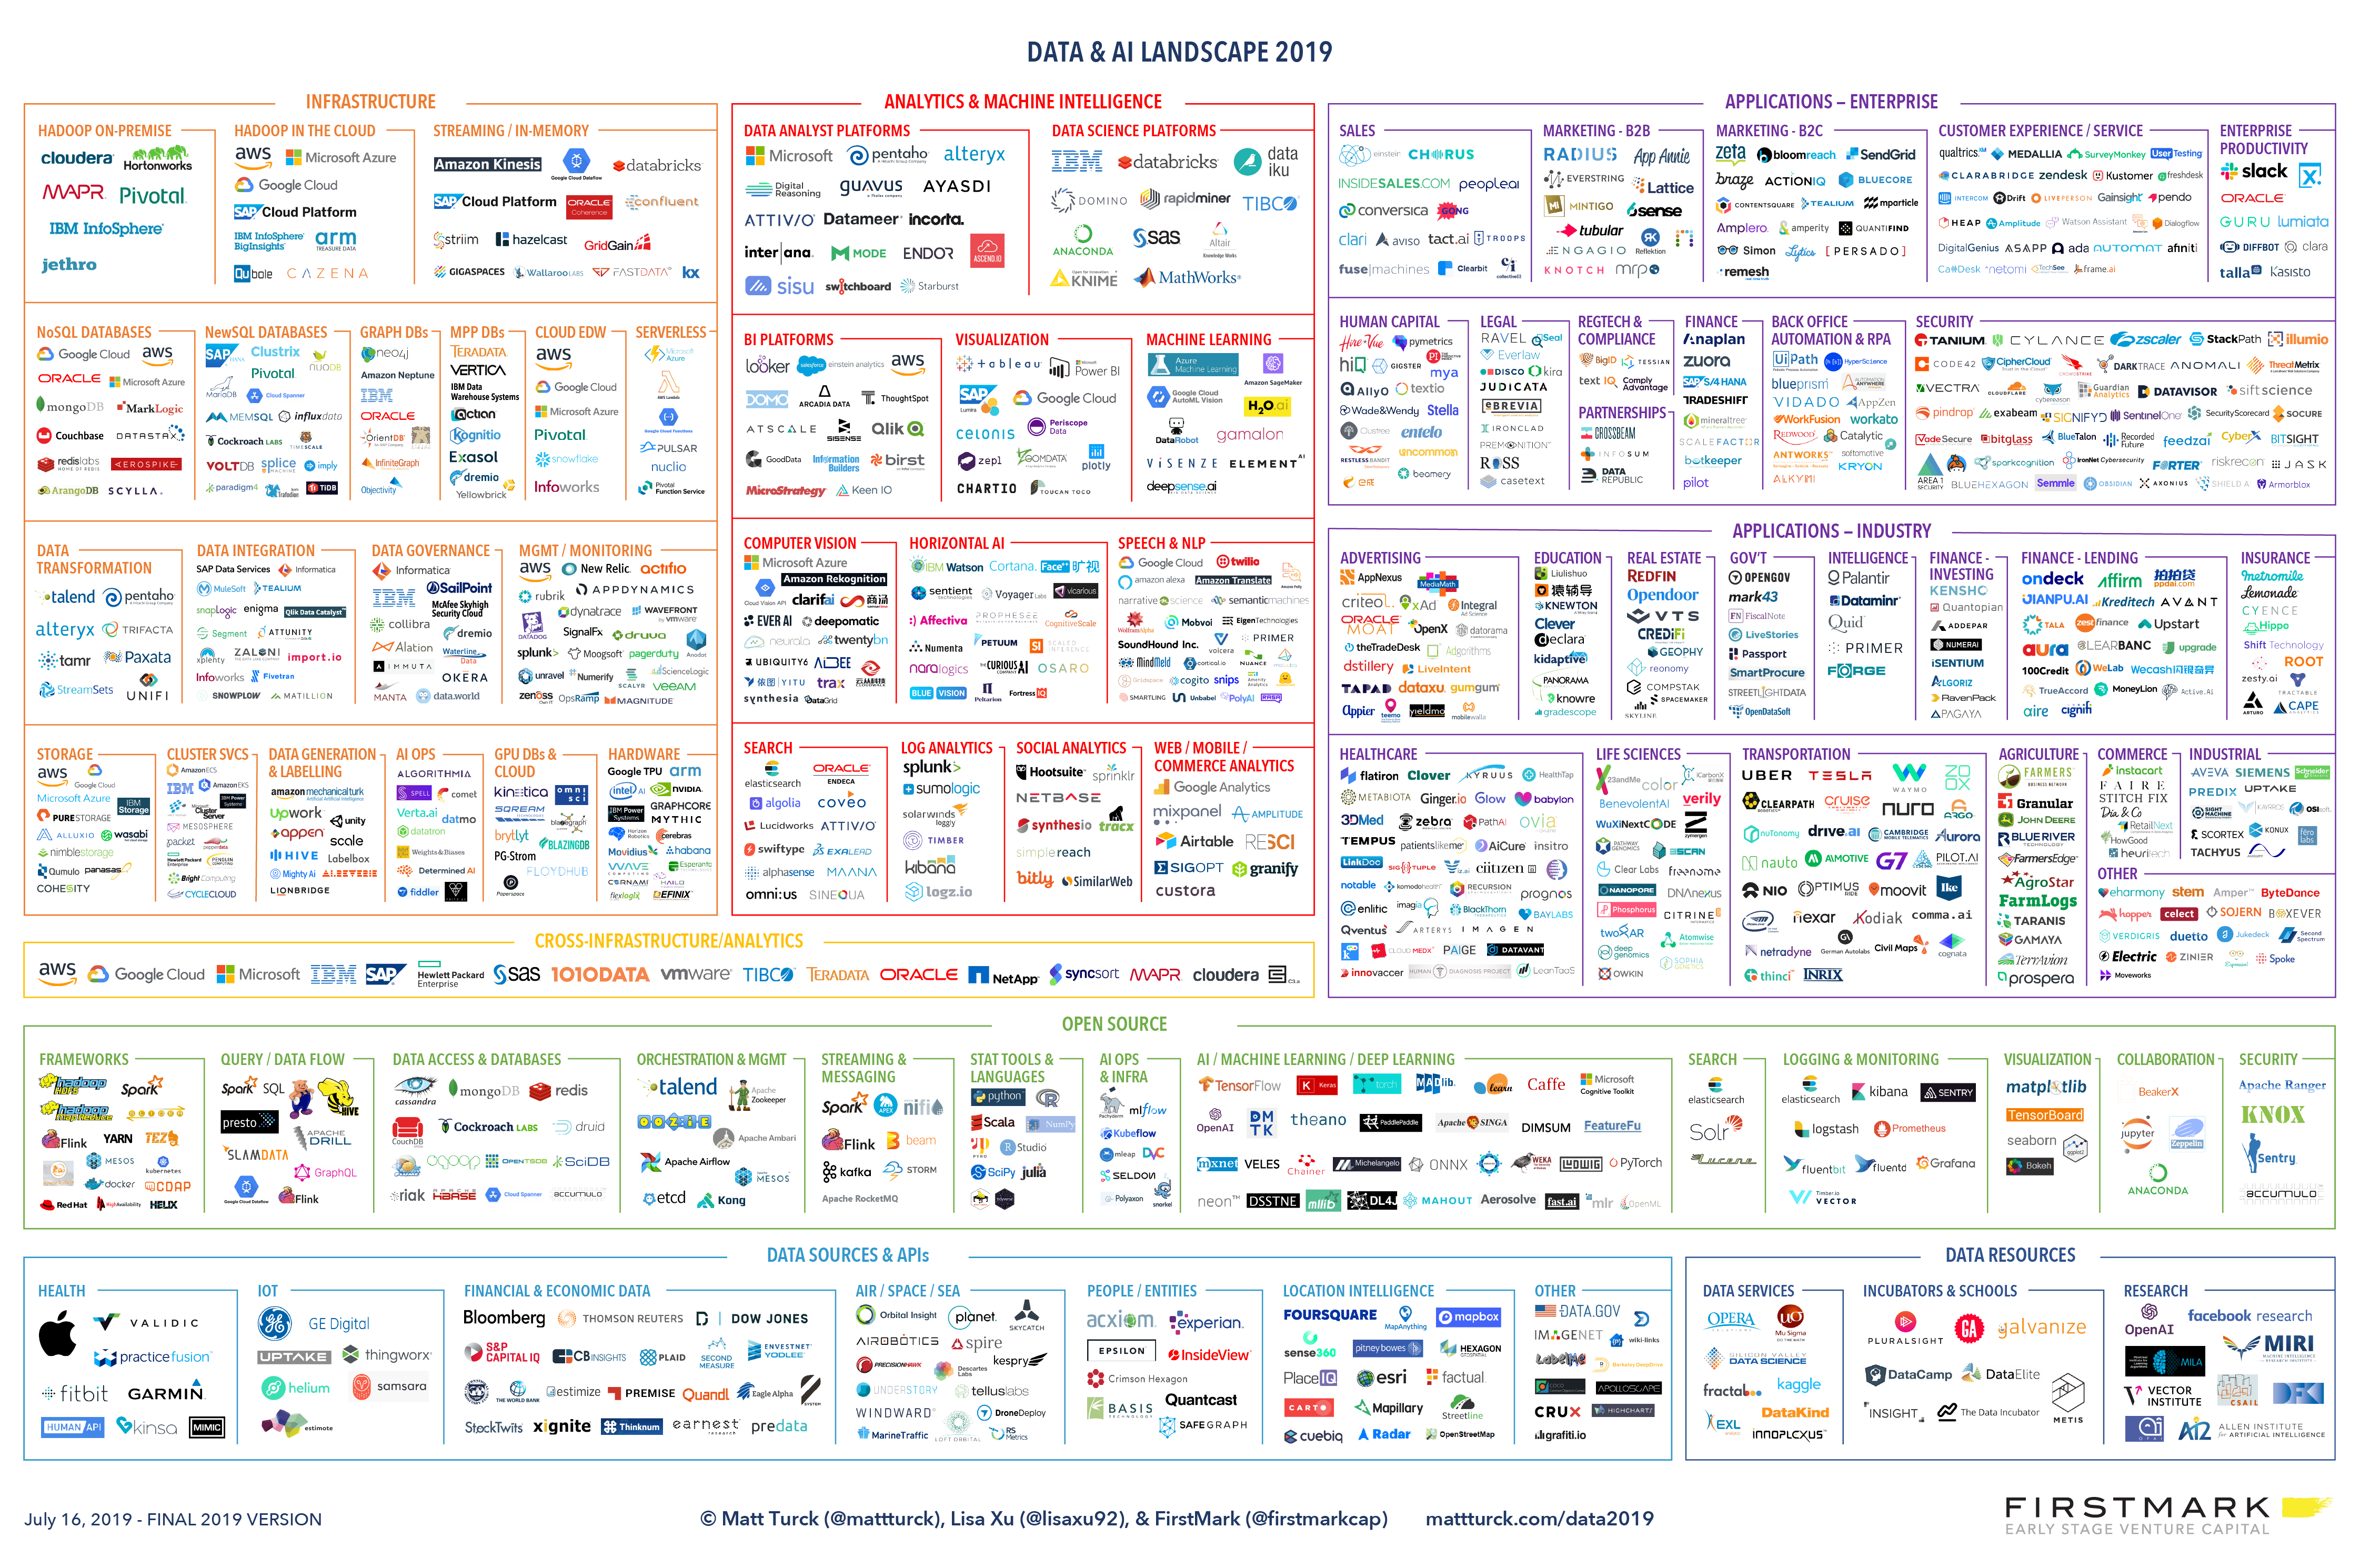
\includepdf[pages=-,angle=90]{landscape.pdf}
    \end{landscape}
\KOMAoptions{paper=a4}
\recalctypearea


\chapterimage{capitulos.pdf}
\chapter{\emph{Gartner Scores}}
\label{anexo-tabelacc}

%A próxima página apresenta tabela\footnote{A tabela original do \relatorioGCC \xspace é chamada de ``\emph{Table 2: Product/Service Rating on Critical Capabilities}.''} contendo a atribuição de notas (\emph{scores}) para cada fornecedor avaliado (horizontal) para cada uma das 15 áreas de capacidade (vertical). 

A próxima página apresenta tabela elaborada a partir do \relatorioGCC contendo a atribuição de notas (\emph{scores}) para cada fornecedor avaliado (horizontal) de cada uma das 15 áreas de capacidade (vertical).

As notas variam de $1,0$ a $5,0$ e apresentam o seguinte significado:

\begin{itemize}
    \item \textbf{1 = Fraco ou ausente}: a maioria ou todos os requisitos definidos para uma capacidade não são alcançados;   
    \item \textbf{2 = Regular}: alguns requisitos não são alcançados;
    \item \textbf{3 = Bom}: atende aos requisitos;
    \item \textbf{4 = Excelente}: atende ou excede alguns requisitos;   
    \item \textbf{5 = Excelente}: excede significativamente os requisitos;
\end{itemize}

Os resultados dos casos de uso construídos no ``\autoref{cap-casos-gartner} -- \nameref{cap-casos-gartner}'' da ``\autoref{parte-estudosdecaso} -- \nameref{parte-estudosdecaso}'' são obtidos pela soma da multiplicação dos pesos definidos para cada área de capacidade e as notas atribuídas a cada fornecedor de acordo com essa tabela. 
\thispagestyle{empty}
\begin{landscape}
    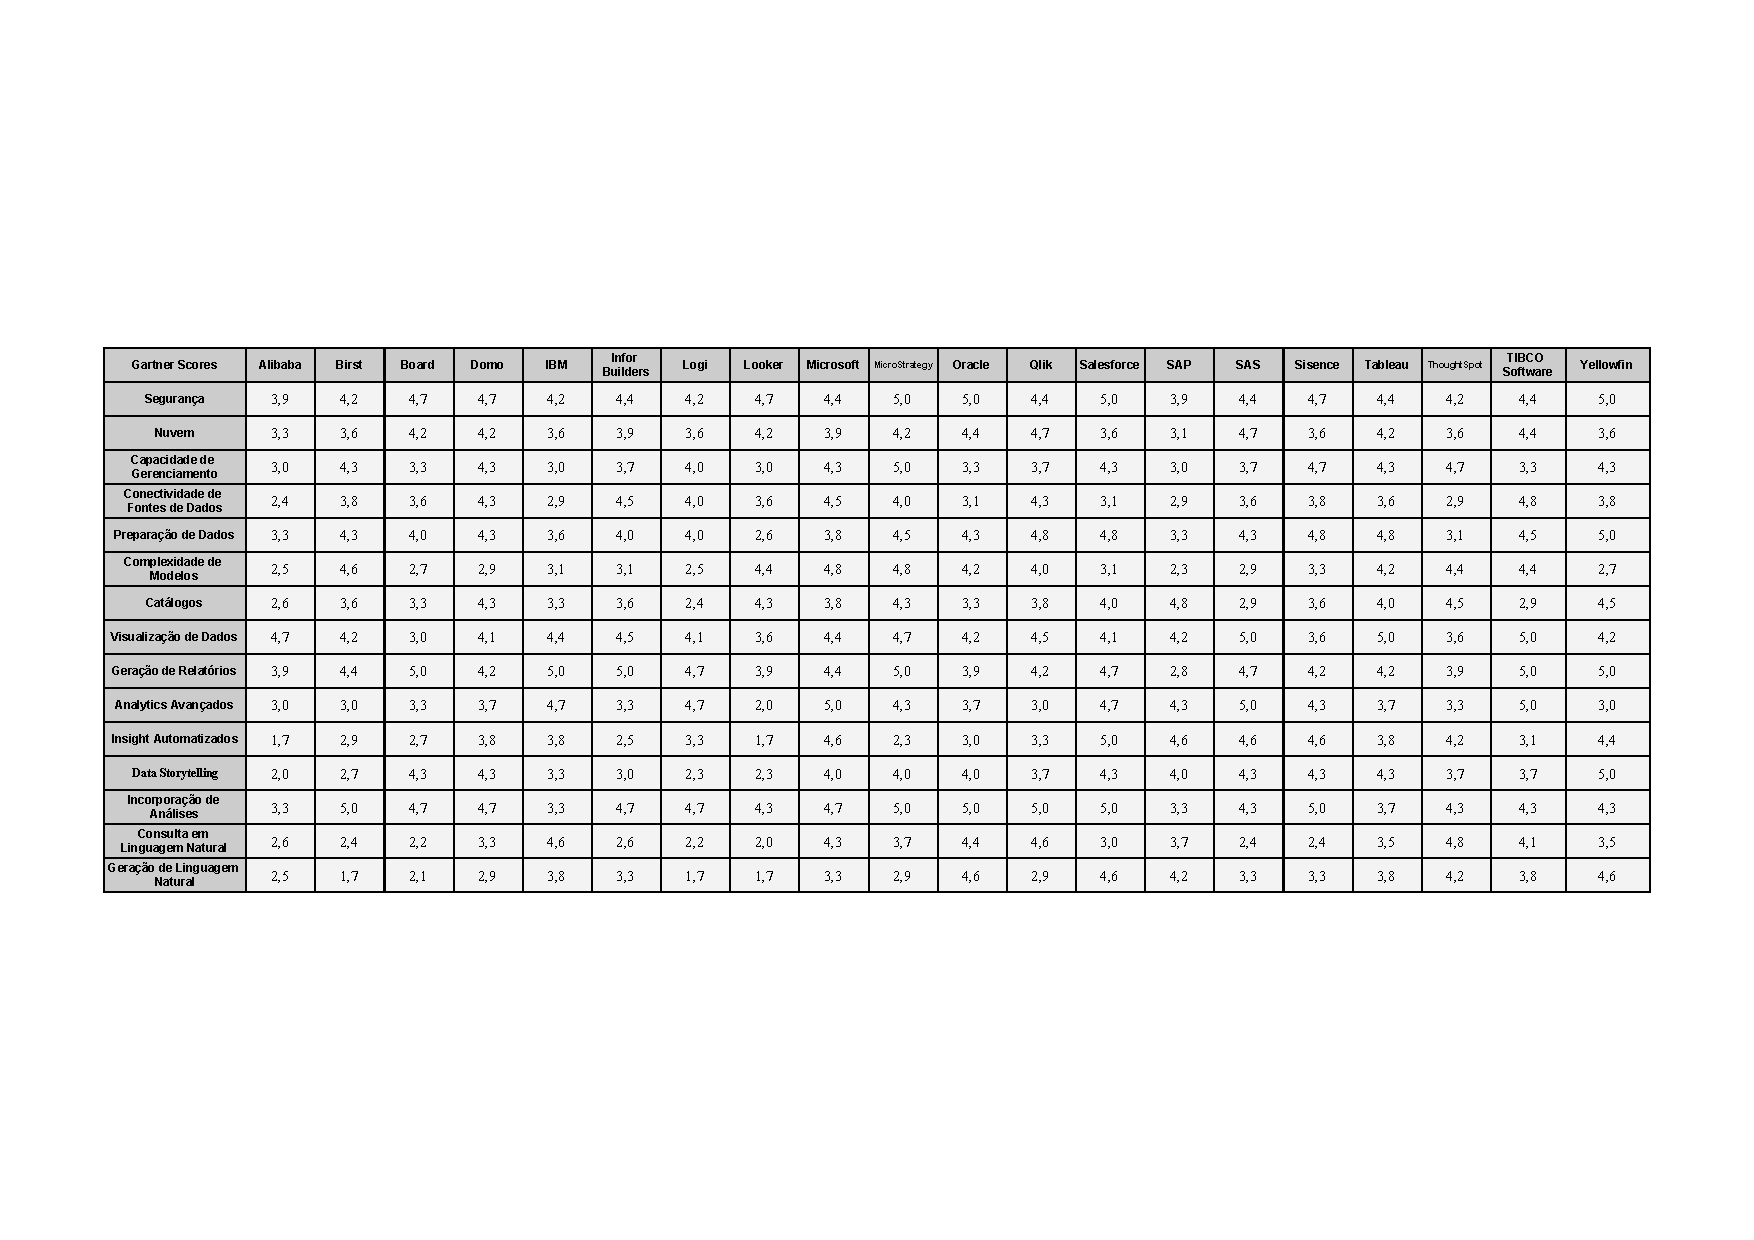
\includepdf[pages=-,angle=90]{gartner.pdf}
\end{landscape}

\chapterimage{capitulos.pdf}
\chapter{\emph{Forrester Scores}}
\label{anexo-tabelafw}

%A próxima página apresenta tabela\footnote{A tabela original do \relatorioFCM \xspace é chamada de ``\emph{FIGURE 2 Forrester WaveTM: Enterprise BI Platforms (Client-Managed) Scorecard, Q3 2019}.''} contendo a atribuição de notas (\emph{scores}) para cada fornecedor avaliado (horizontal) para cada um dos critérios (vertical).

A próxima página apresenta tabela elaborada a partir do \relatorioFCM contendo a atribuição de notas (\emph{scores}) para cada fornecedor avaliado (horizontal) de cada um dos critérios (vertical). De forma semelhante ao anexo anterior, essas notas avaliam os requisitos na escala de $1,0$ a $5,0$.

Os resultados dos casos de uso construídos no ``\autoref{cap-casos-forrester} -- \nameref{cap-casos-forrester}'' da ``\autoref{parte-estudosdecaso} -- \nameref{parte-estudosdecaso}'' são obtidos pela soma da multiplicação dos pesos definidos para cada critério e as notas atribuídas a cada fornecedor de acordo com essa tabela. 

\thispagestyle{empty}
\begin{landscape}
    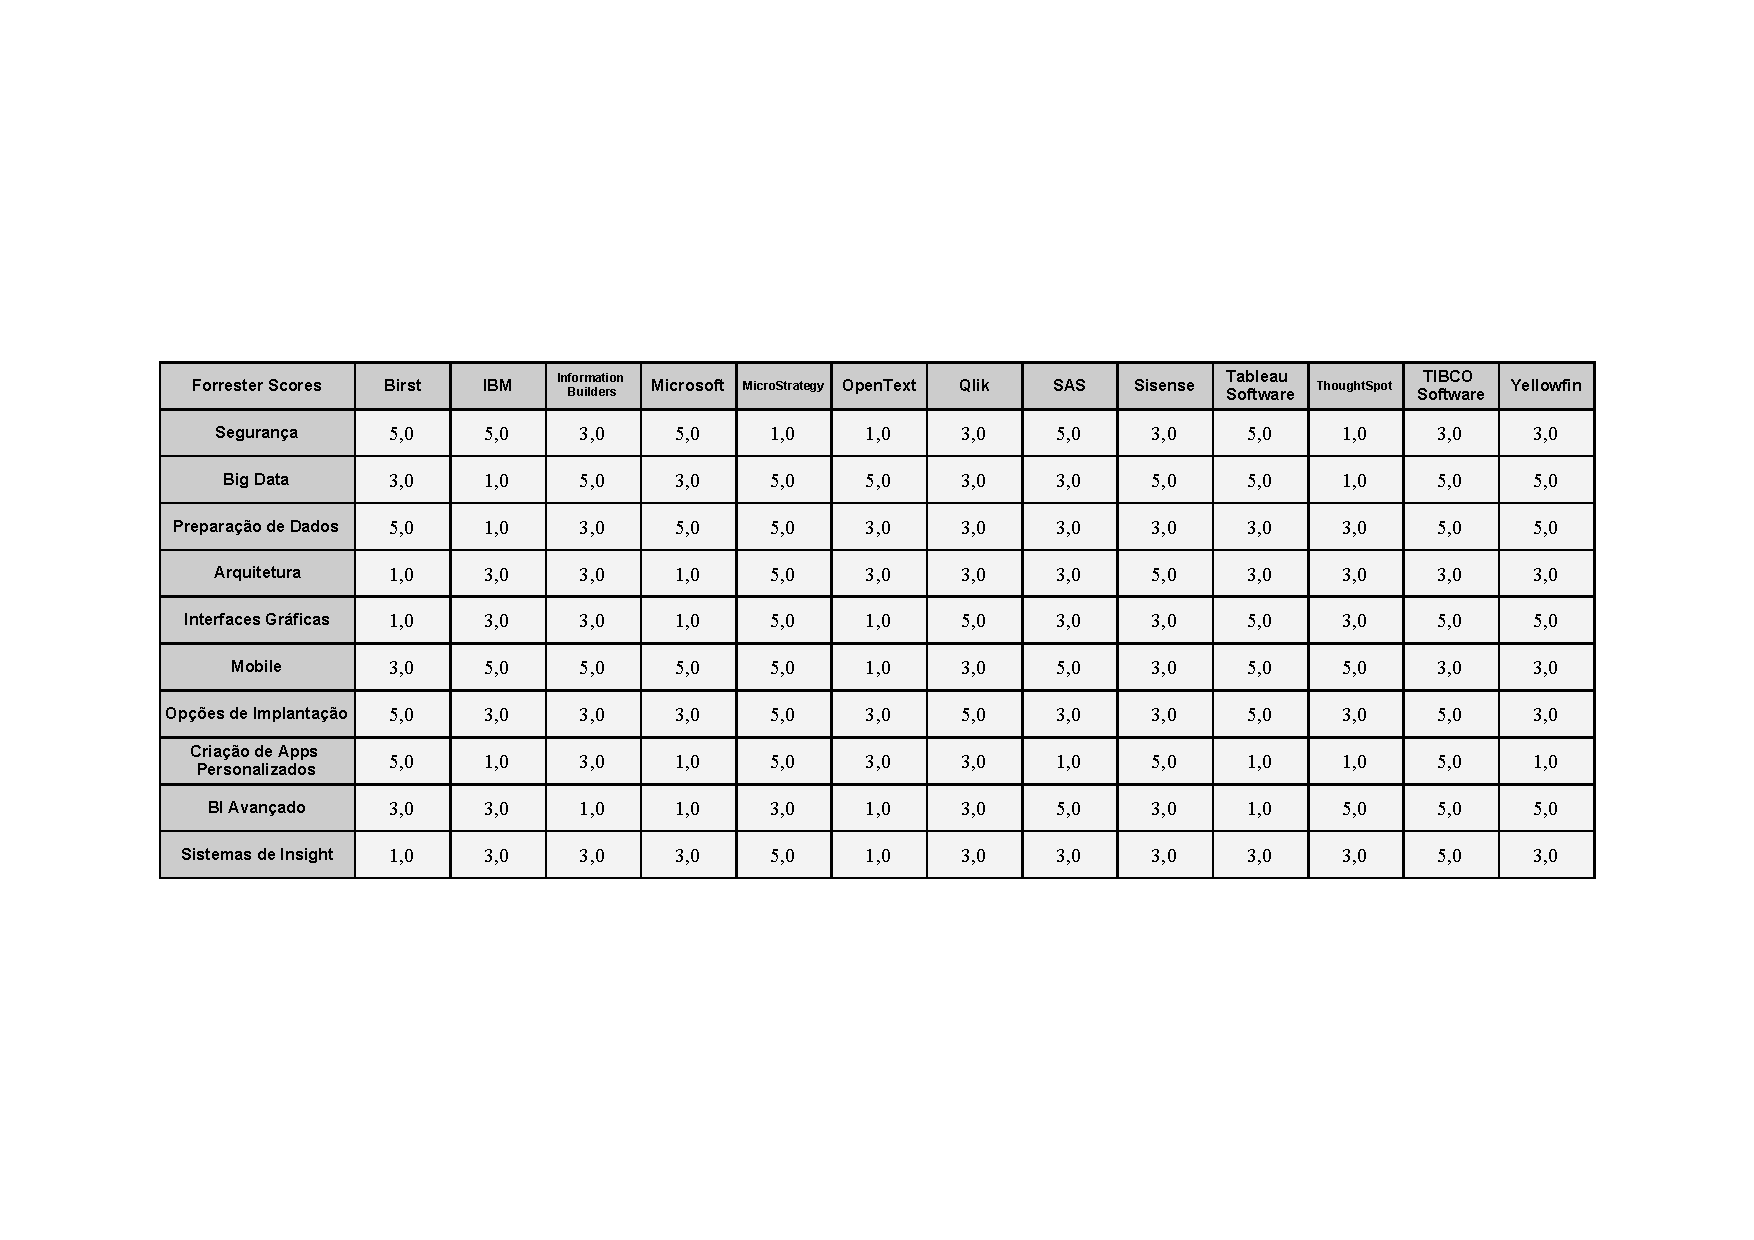
\includepdf[pages=-,angle=90]{forrester.pdf}
\end{landscape}



% ----

\end{document}
